%% document
\documentclass[11pt]{article}
\usepackage[letterpaper, portrait, margin=0.75in]{geometry}
\usepackage{setspace}
\usepackage{color}

% text
\usepackage[utf8]{inputenc}
\setlength\parindent{0pt}
\setlength{\parskip}{1em}
\renewcommand{\familydefault}{\sfdefault}
\newcommand{\RomanNumeral}[1]{\textrm{\uppercase\expandafter{\romannumeral #1\relax}}}

% math
\usepackage{amssymb}
\usepackage{amsmath}
\usepackage[cm]{sfmath}
\usepackage{commath}
\usepackage{multirow}
\DeclareMathAlphabet{\mathpzc}{OT1}{pzc}{m}{it}

% graphics
\usepackage{graphics}
\usepackage{graphicx}
\usepackage{epsfig}
\usepackage{epstopdf}
\usepackage{xpatch}
\usepackage{pdfpages}
\usepackage{float}

% each section begins new page
\let\stdsection\section
\renewcommand\section{\clearpage\stdsection}

% hyperref
\usepackage[colorlinks=true, linkcolor=black, urlcolor=blue, citecolor=black, anchorcolor=black]{hyperref}
\usepackage[all]{hypcap}  % helps hyperref work properly



\usepackage[shortlabels]{enumitem}
\setlist[enumerate, 1]{nosep}
\setlist[enumerate, 2]{nosep, topsep=-5ex}
\setlist[enumerate, 3]{nosep, topsep=-5ex}
\setlist[enumerate, 4]{nosep, topsep=-5ex}
\setlist[itemize, 1]{nosep}
\setlist[itemize, 2]{nosep, topsep=-5ex}
\setlist[itemize, 3]{nosep, topsep=-5ex}
\setlist[itemize, 4]{nosep, topsep=-5ex}

% bibliography
\usepackage[numbers]{natbib}

% title
\title{Wisconsin Photoreactor \\ Assembly Instructions}
\author{
  Philip Lampkin \\
  Blaise J. Thompson \\
  Samuel H. Gellman
  }
\date{\today}

\begin{document}

\maketitle


\includegraphics[width=\textwidth]{"../coverart.jpg"}

\tableofcontents

\section{Introduction}

The Wisconsin Photo-Reactor (WPR) is made to be easily assembled.
This document is meant to help chemists accomplish this assembly.
Each reactor has two major components requiring detailed custom assembly:

\begin{itemize}
  \item The 3D printed enclosure, described in \autoref{SEC:enclosure}
  \item The drive electronics, described in \autoref{SEC:electronics}
\end{itemize}

With these two major components complete, assembly of the WPR is relatively straight-forward.
Details of final assembly are described in \autoref{SEC:assembly}.

Throughout this document we refer to an online repository containing source and design files.
This repository appears at \url{https://github.com/uw-madison-chem-shops/wisconsin-photoreactor}.
This repository contains everything including the source for this very document.

A working WPR is made up of many separate commercially available parts.
This guide assumes that you have already done the work of procuring those parts.
The online repository contains several README files with detailed part numbers and suggested vendors.

The WPR is a living project.
We welcome and encourage duplication and modification of our designs and documentation.
If you notice problems or omissions within this assembly document, please consider opening an issue or pull request.

\section{3D Printed Enclosure} \label{SEC:enclosure}

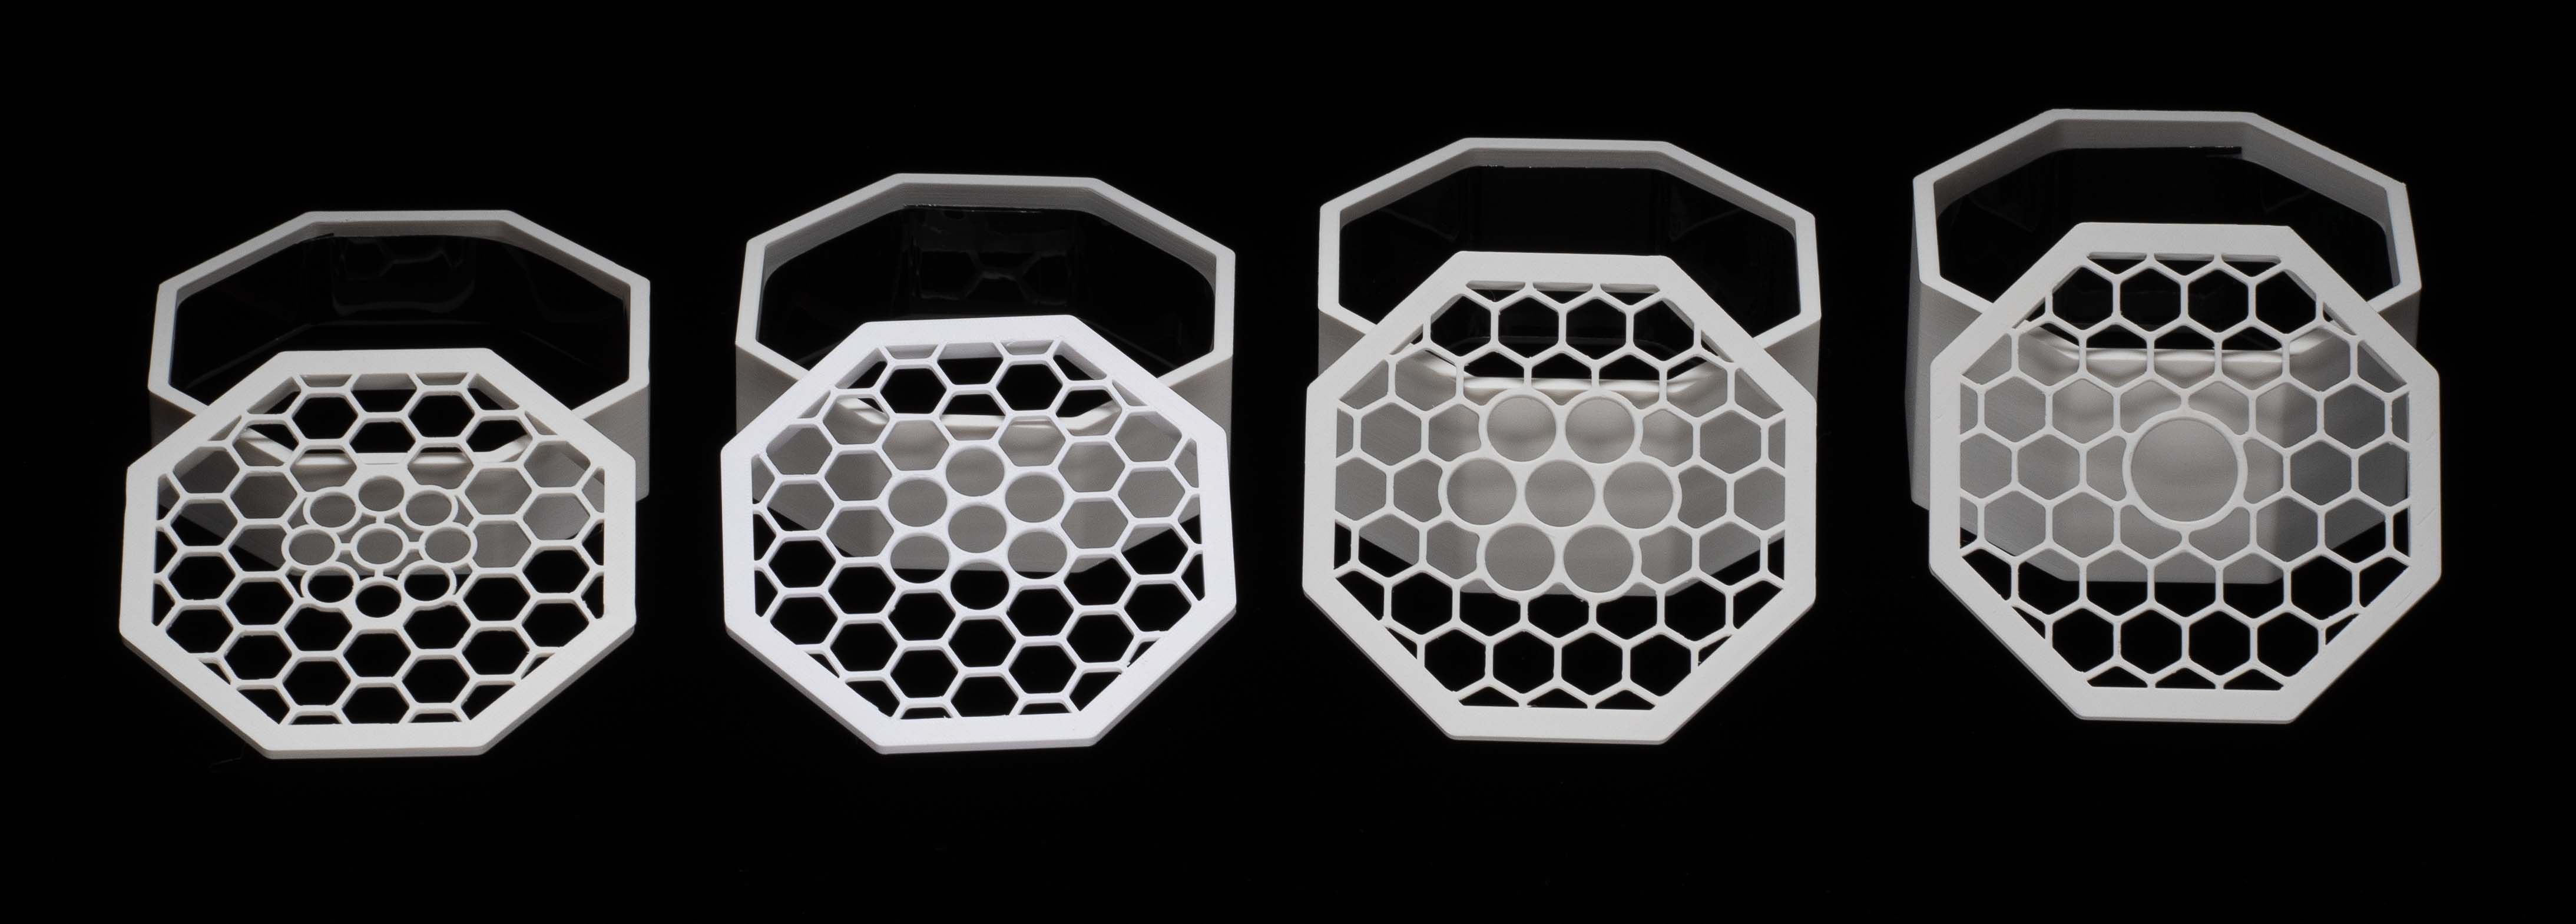
\includegraphics[width=\textwidth]{"./3dp-coverat.jpg"}

The body of the WPR is made up of three main pieces:

\begin{itemize}
    \item Base, containing LEDs, fan, and drive electronics.
    \item Top plate accepting reaction vials.
    \item Chamber walls spacing the top plate at the appropriate distance away from the base.
\end{itemize}

The WPR base is the same for all reactors.
Look within the repository in the subdirectory ``photoreactor-base'' to find design and production files to produce the WPR base.
You will also need to print a cable anchor, see files in that same directory.

The top plate and chamber height must be specified for the particular reaction vessels used.
Four examples for different vial sizes are pictured above.
Look within the repository in the subdirectory ``photoreactor-tops'' to find existing designs.
We encourage you to design your own if none of these suit your application.
Consider adding your new designs to repository so that others may benefit from your design efforts.

When interacting with the design files in our online repository you will see several different filetypes.
We have designed the WPR enclosure using Fusion 360, and have included those f3d design files for those that wish to extend or modify the designs.
Interacting with f3d files will require a Fusion 360 license.
You will also find stl files in the online repository.
These are common 3D-model exchange files which can be viewed using any 3D modeling program.
In fact, GitHub itself has a built in stl viewer which you may use to inspect our designs.

There are many options for getting your enclosures printed.
We recommend white PLA as a material, although any white material should work---we have also used ABS.
If you are printing yourself, follow the instructions provided by your printer to produce slices and program your printer.
Note that you will need support material for the base.
Any company or shop offering 3D printing as a service should be able to accept our stl files without further modification.

We have succesfully printed using the following printers:

\begin{itemize}
  \item Ender 3
  \item Stratasys uPrint SE Plus
  \item Ultimaker 3
\end{itemize}

Once your parts are done you may need to remove extra bonding material with a razor blade or exacto-knife.
The three pieces of your reactor should fit together snugly and securely.

\clearpage

\begin{center}
  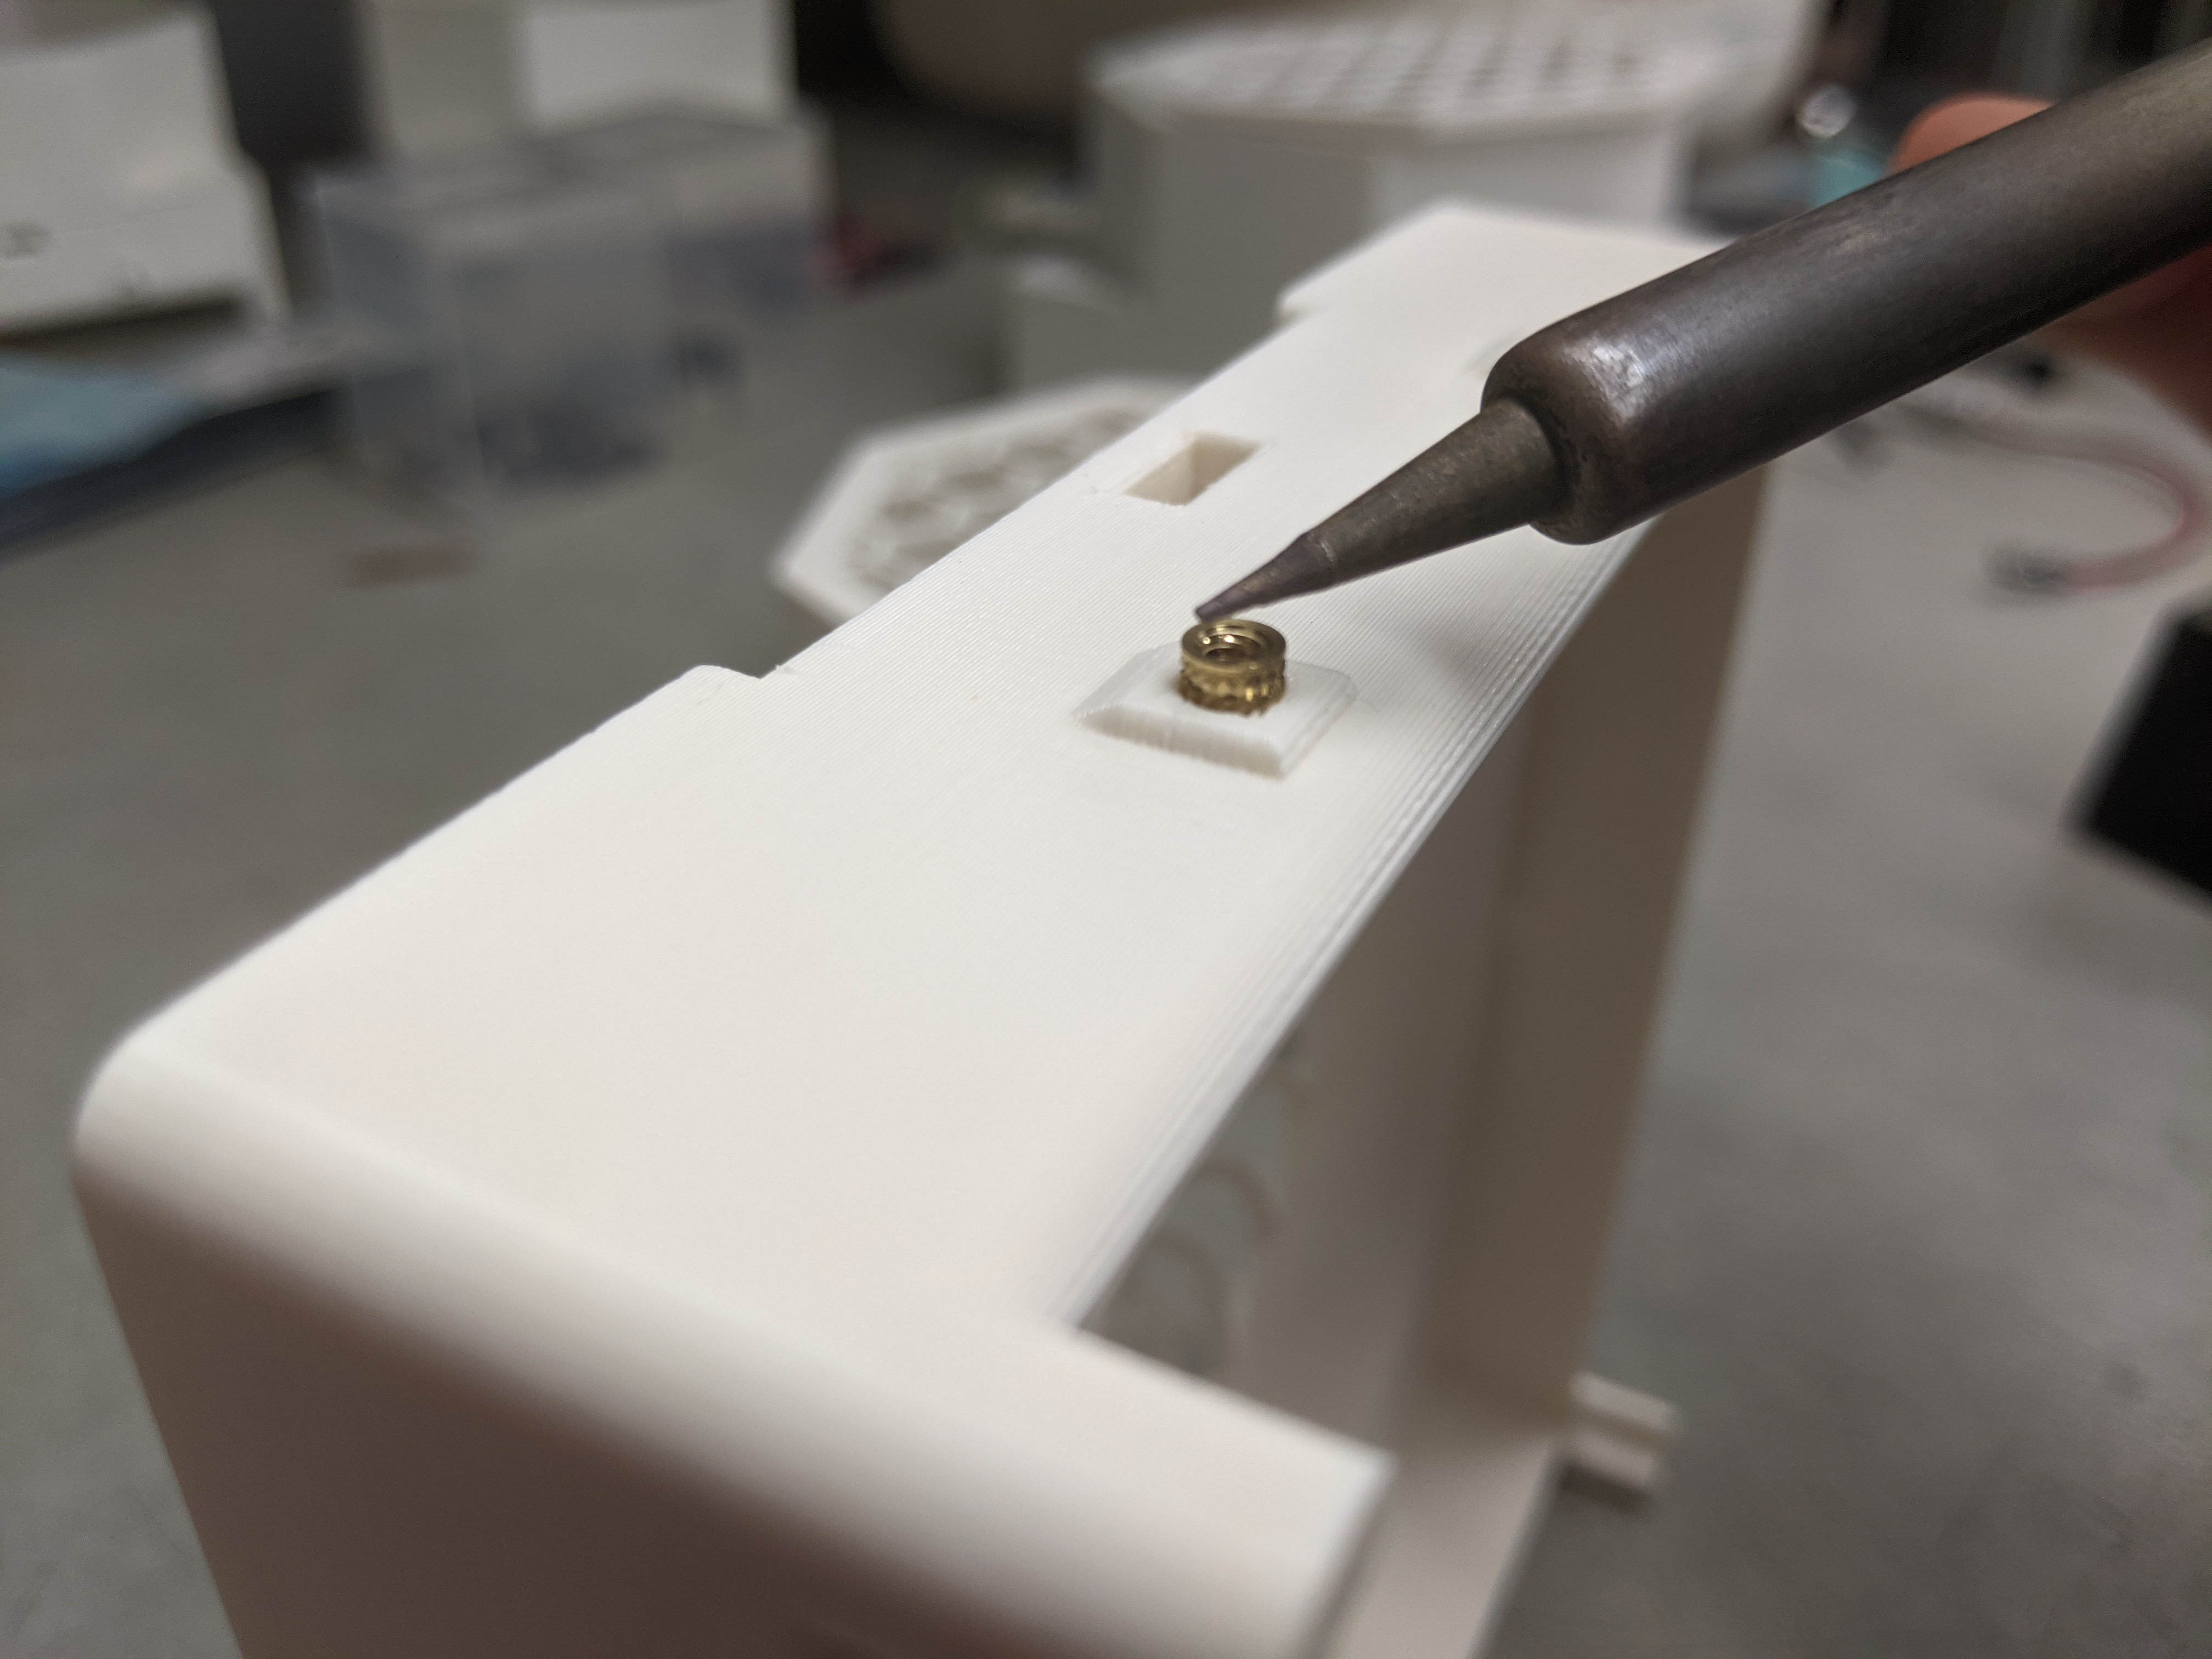
\includegraphics[width=0.5\textwidth]{"./heat-insert.jpg"}
\end{center}

Each WPR base contains seven threaded heat inserts.
These allow components such as the drive circuit board to rigidly attach to the base via machine screws.
Use a soldering iron to carefully heat these while pushing them into their cavities.

\section{Electronics} \label{SEC:electronics}

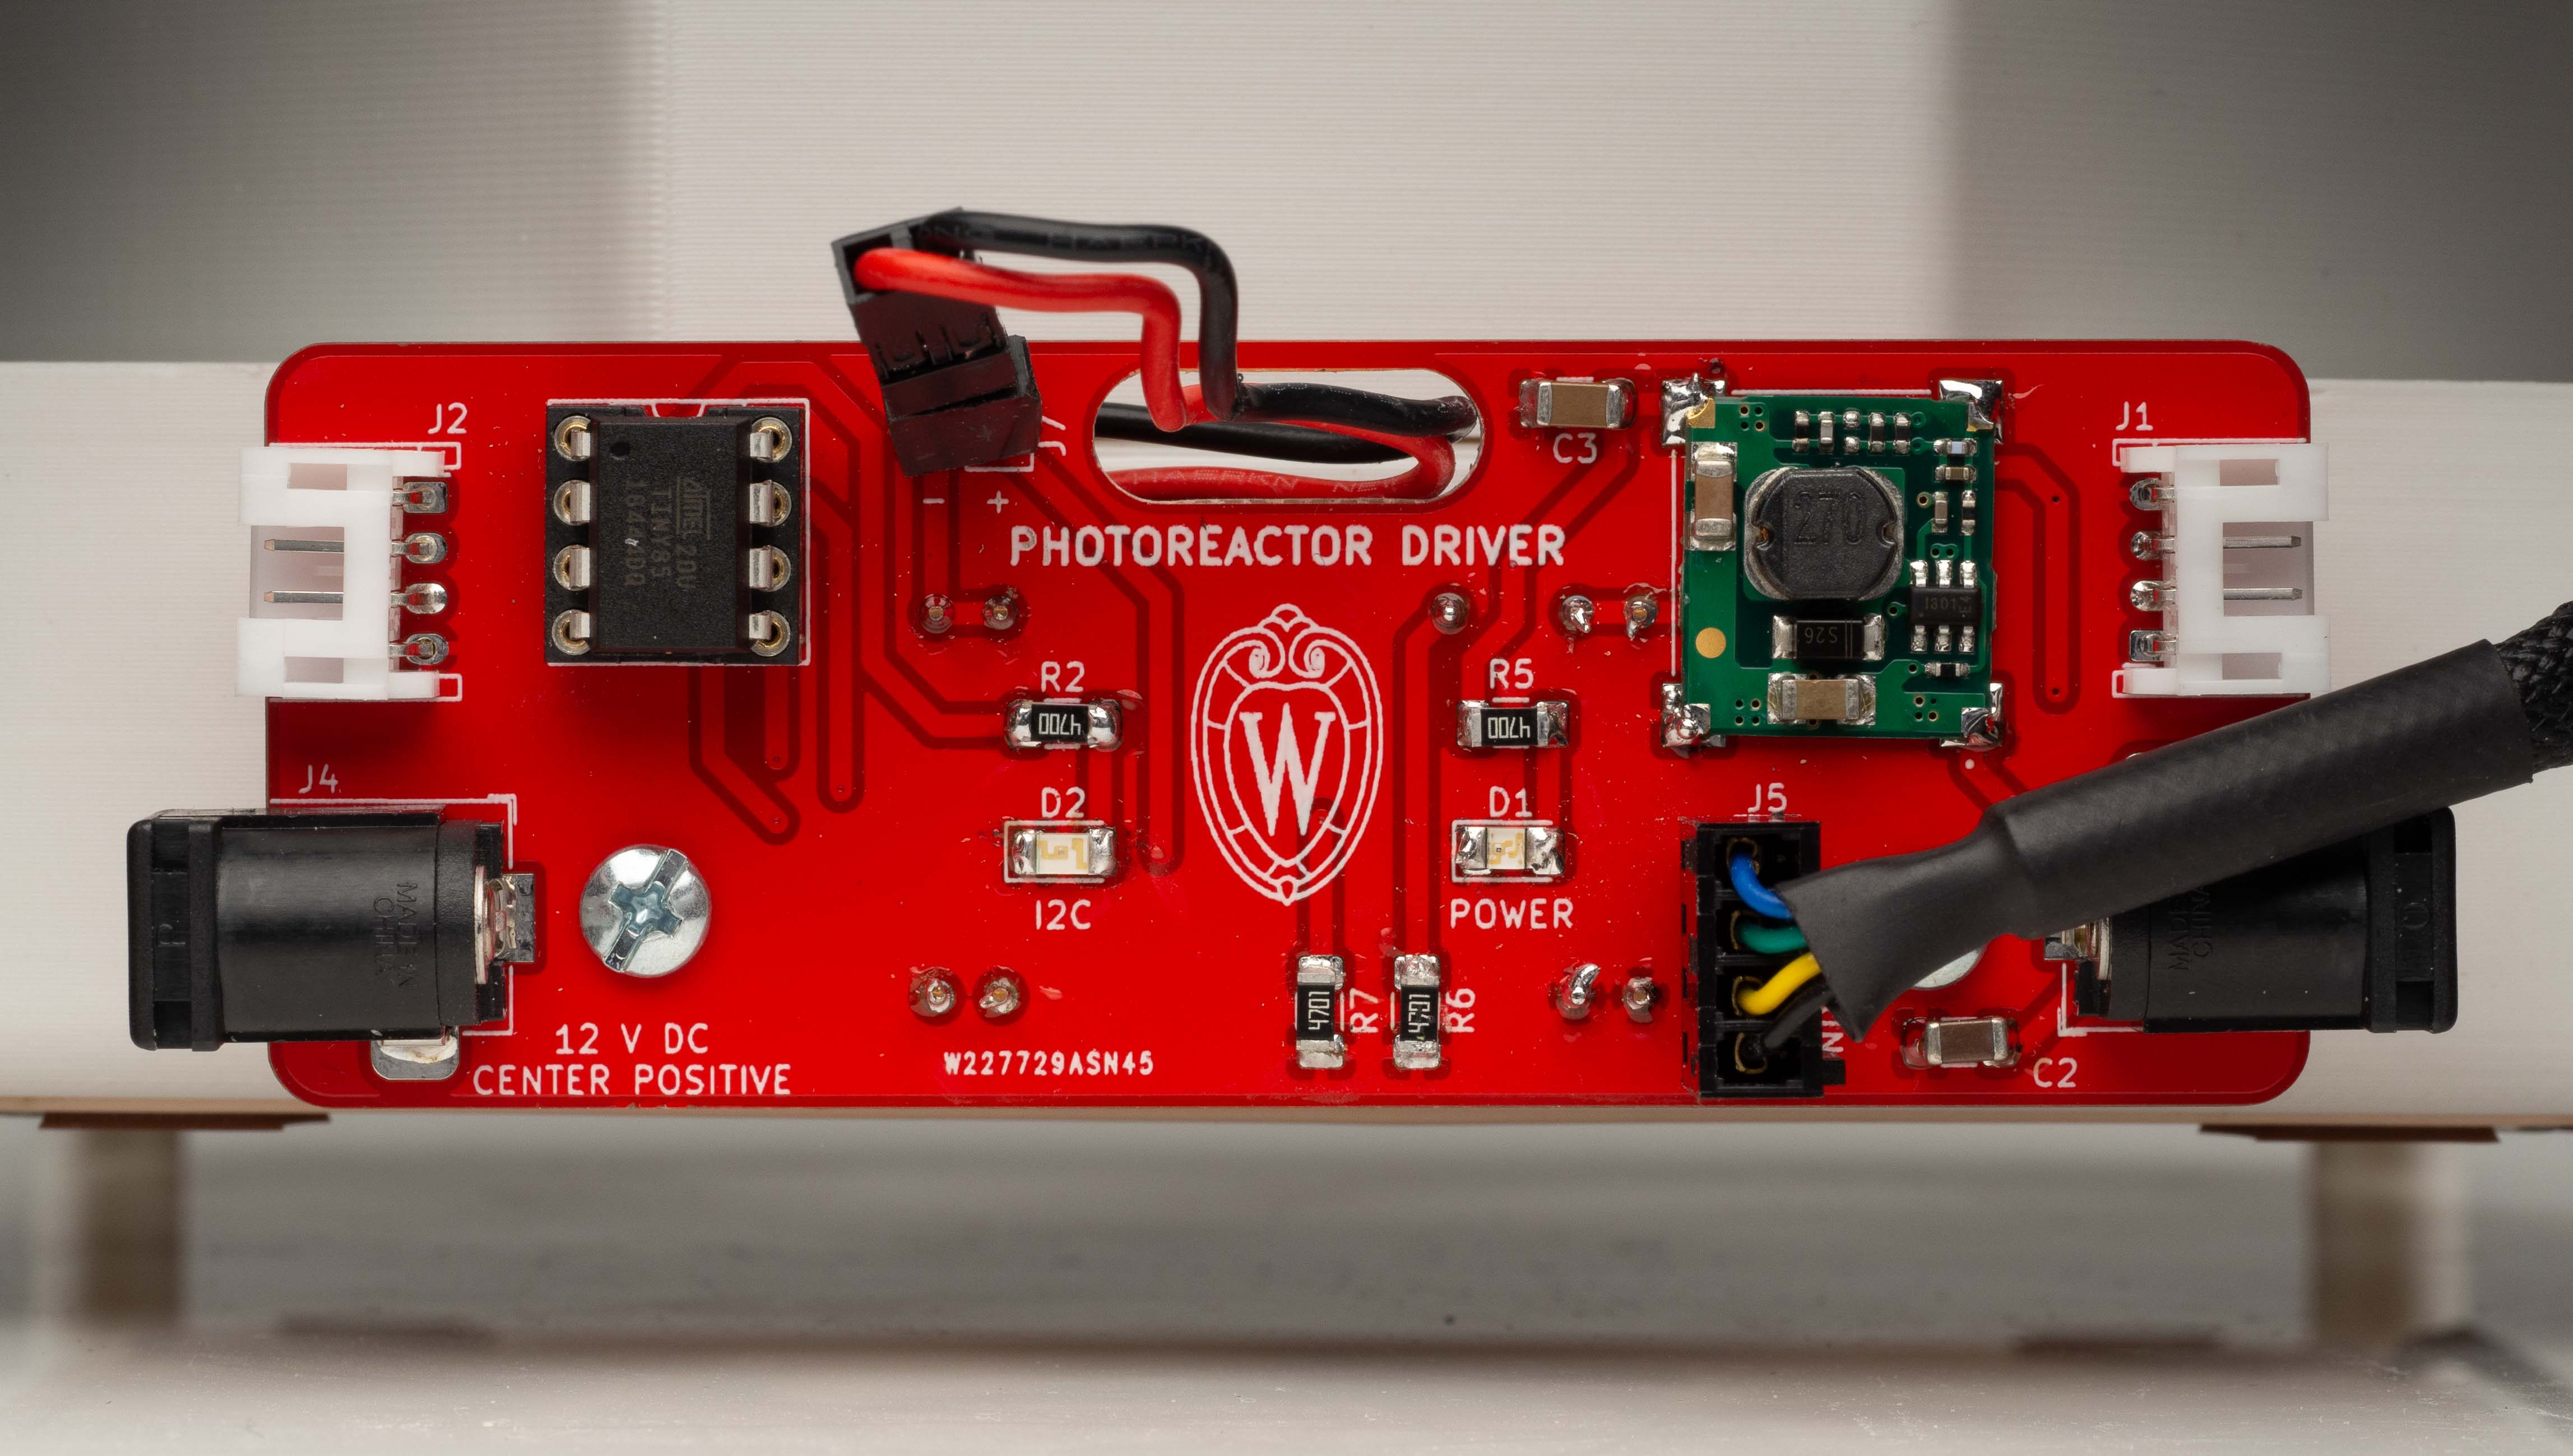
\includegraphics[width=\textwidth]{"./electronics-coverart.jpg"}

The WPR incorporates small circuit boards controlling the incorporated LED and fan.
We refer to these small boards as ``drivers''.
There are two types available: the ``analog-driver'' and ``digital-driver''.
Refer to the associated directories in the online repository for design files for each of these.

Both drivers are built around Mean Well's LDD-1000L LED driver module.
This module delivers constant current up to one amp.
The current delivered can be controlled electronically in several different ways.
WPR users wishing to understand this design should refer to Mean Well's datasheet.

The analog-driver circuit is made to be as simple as possible.
The circuit accepts DC 12 V through a barrel jack.
A small knob is used to adjust light intensity.
Fan speed is not adjustable.
Refer to \autoref{SEC:analog-driver} for analog-driver assembly instructions and further explanation.

The digital-driver circuit is made to be incorporated into an I$^2$C-based digital control system.
In addition to power, these boards have 4-pin connectors to carry the I$^2$C serial data.
The digital-driver is pictured above, without any connectors attached.
Refer to \autoref{SEC:digital-driver} for digital-driver assembly instructions and further explanation.

When interacting with the design files in our online repository you will see several different filetypes.
These circuit boards were designed using KiCad, a free and open source electronics CAD software.
All KiCad files are contained within the ``kicad'' subdirectories.
You may modify and extend these designs however you like.

Those wishing to reproduce our designs should refer to the gerber subdirectory.
Within the gerber directory you will find zip files for each separate version of the PCB.
You may upload these zip files to PCB manufacturers when ordering copies of our designs.

\clearpage
\subsection{Analog} \label{SEC:analog-driver}

The analog driver circuit is meant to be as simple as possible while still allowing for reproducible LED intensity control.
To this end, the number of components has been minimized as much as possible.
A full schematic of the analog circuit appears at the end of this section.
A bill of materials appears within the README of the online repository.

\begin{center}
  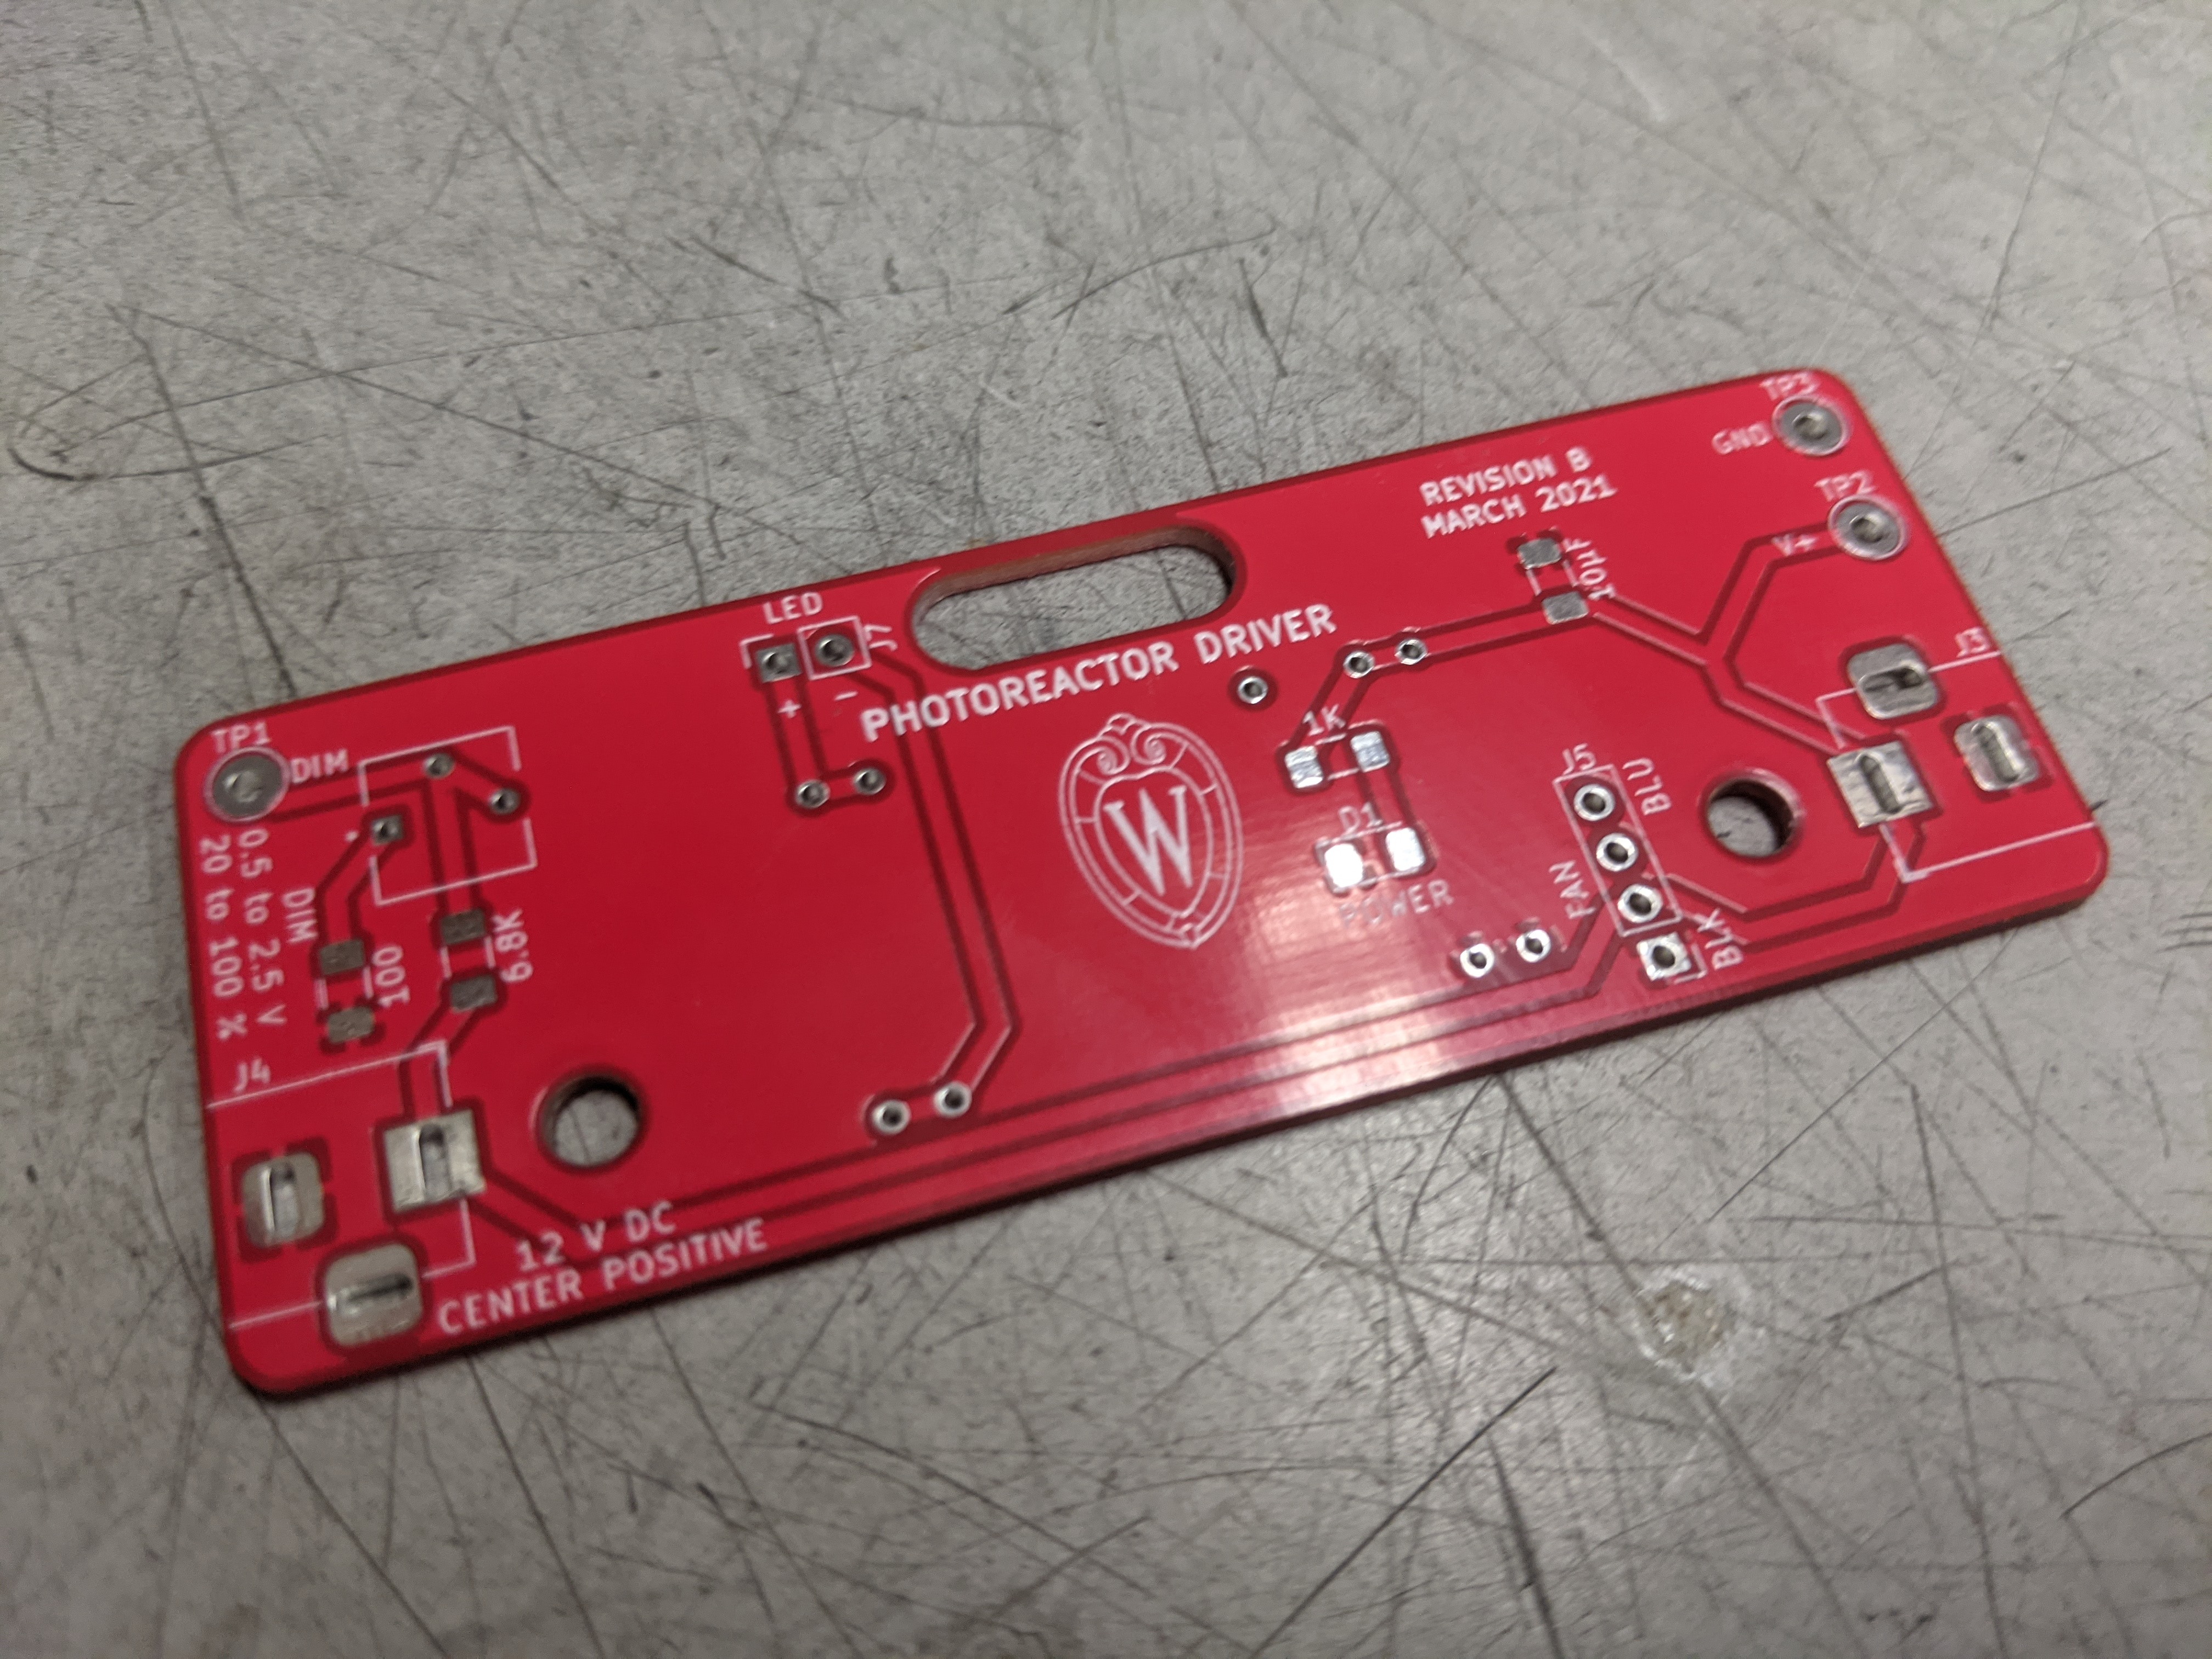
\includegraphics[width=\textwidth/2]{"./bare-pcb.jpg"}
\end{center}

Your PCB manufacturer will send you a bare board, as seen above.

\begin{center}
  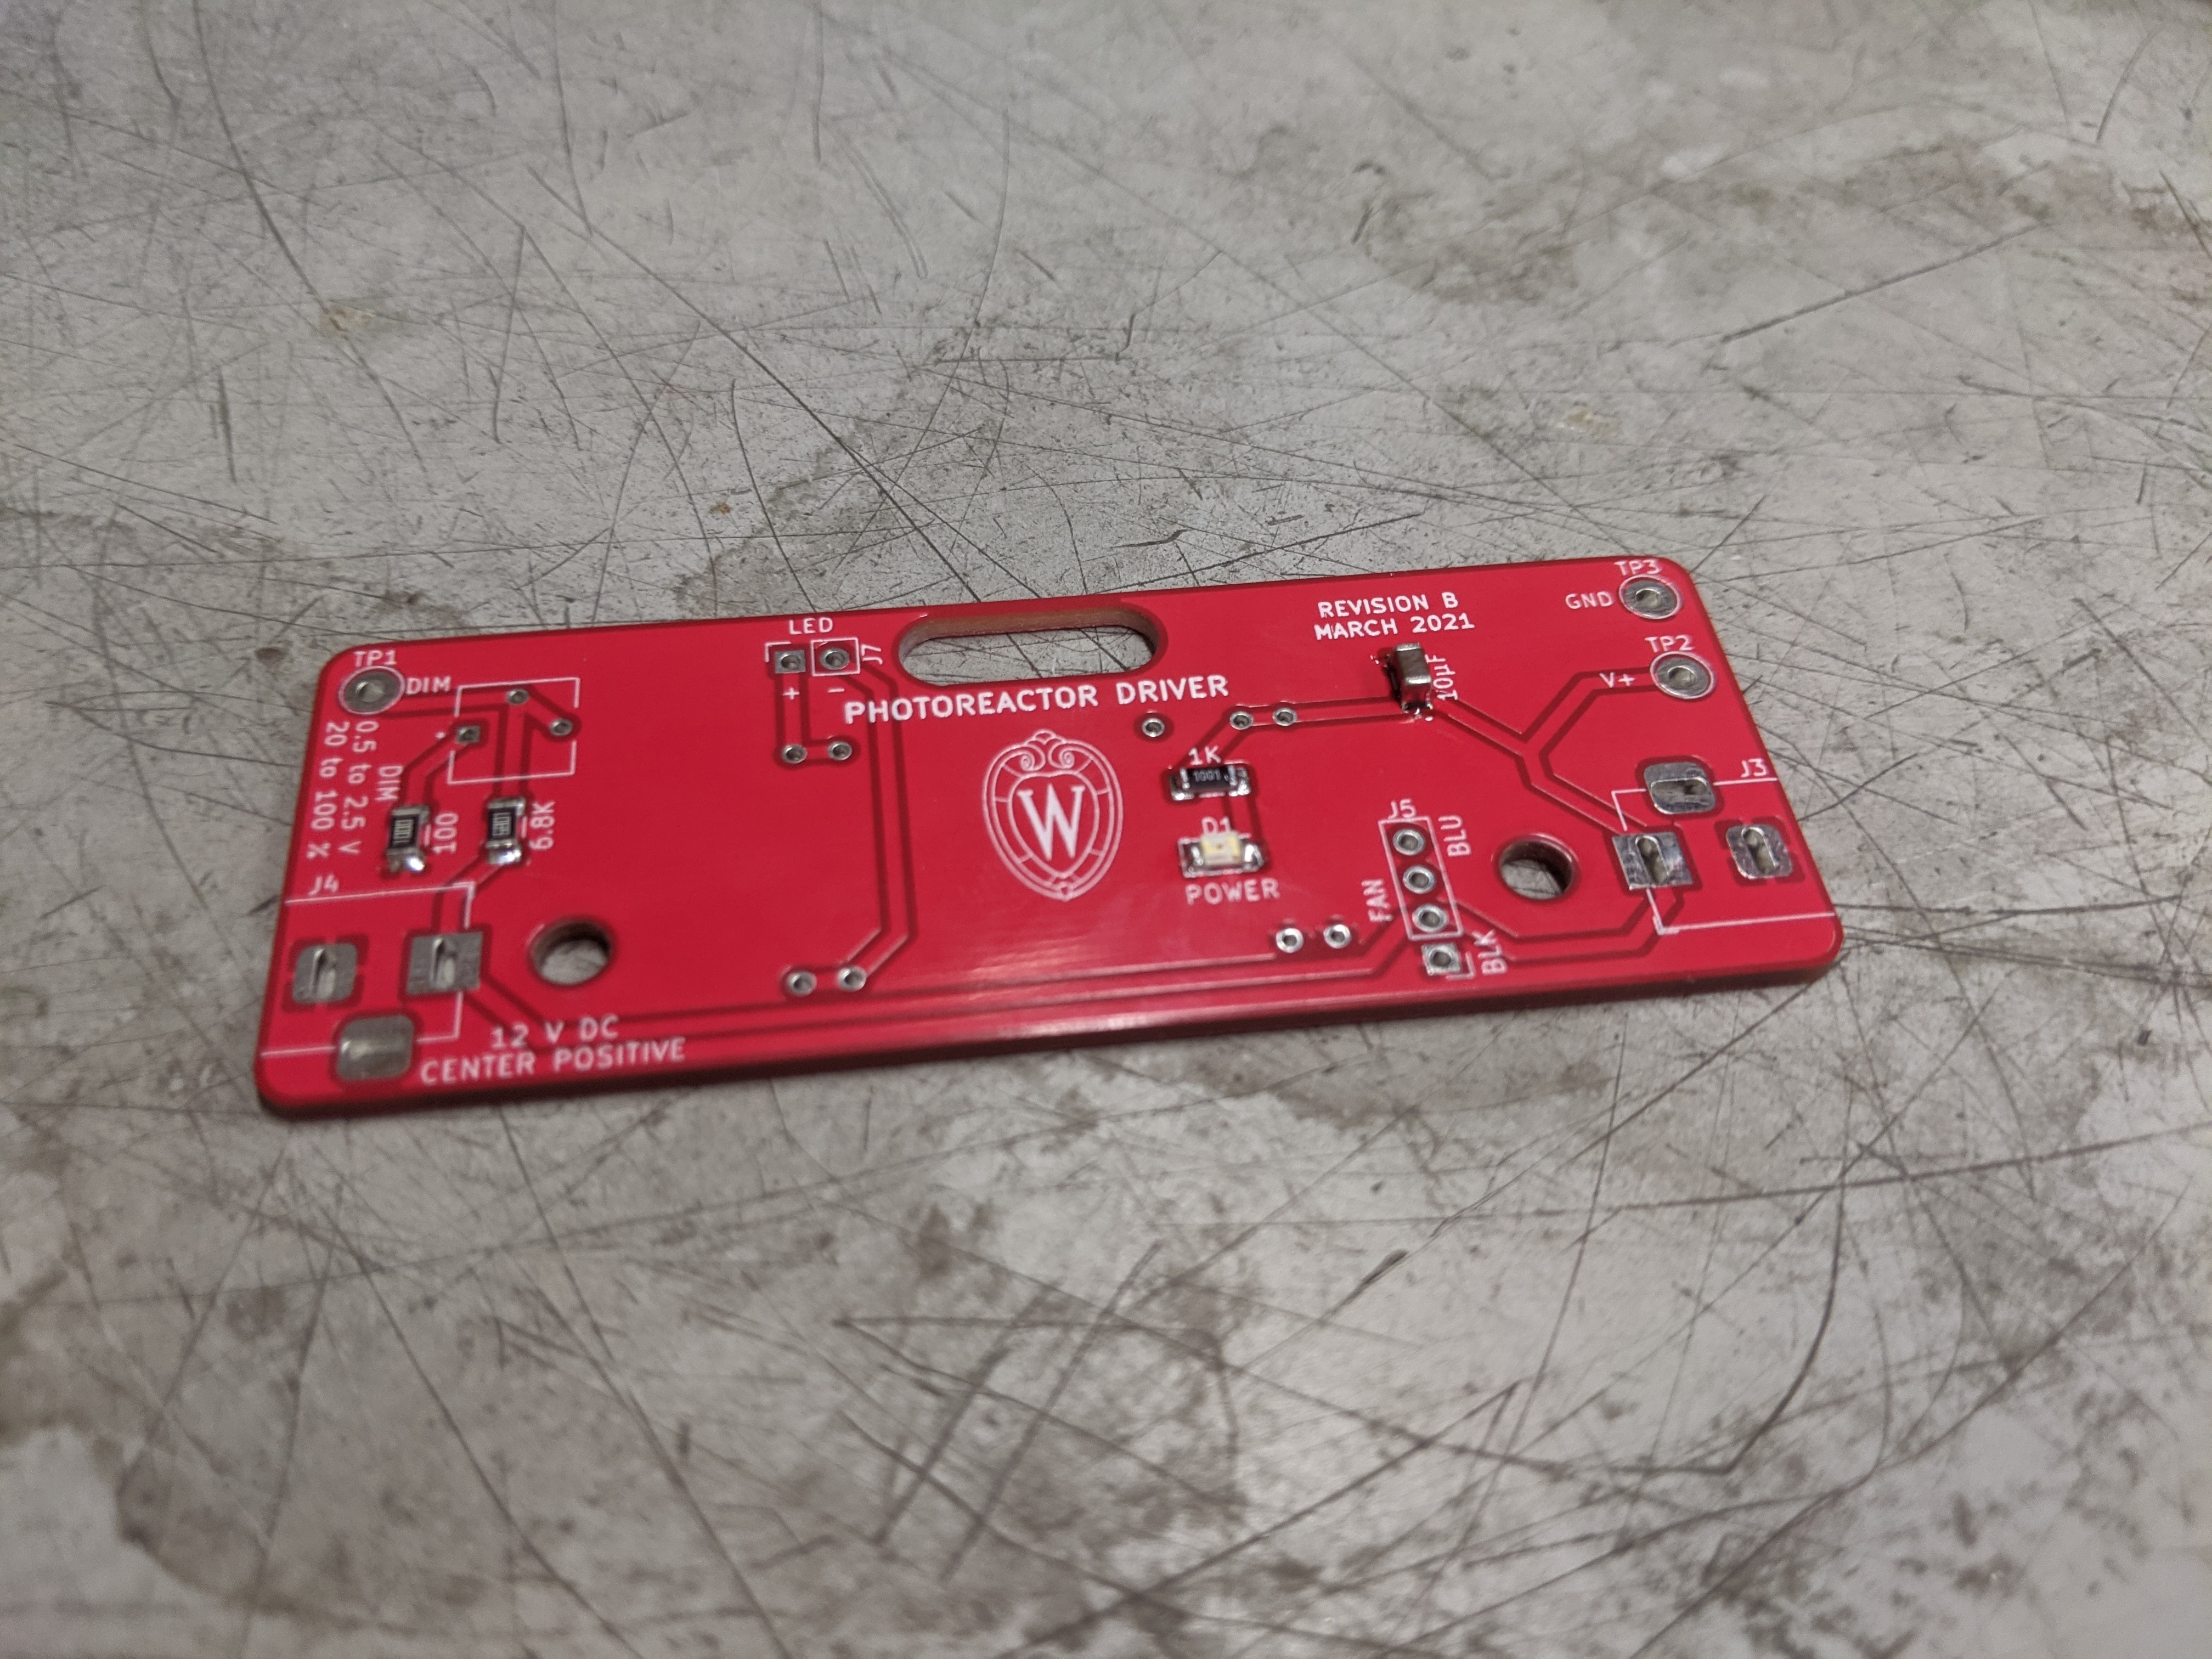
\includegraphics[width=\textwidth/2]{"./surface-mount.jpg"}
\end{center}

Begin by adding the surface mount components.
Recommend thin solder, e.g. 0.015''.
The LED does have a polarity---ensure that the small green line points towards ground (left).
Once done your board should look like the above.

\begin{center}
  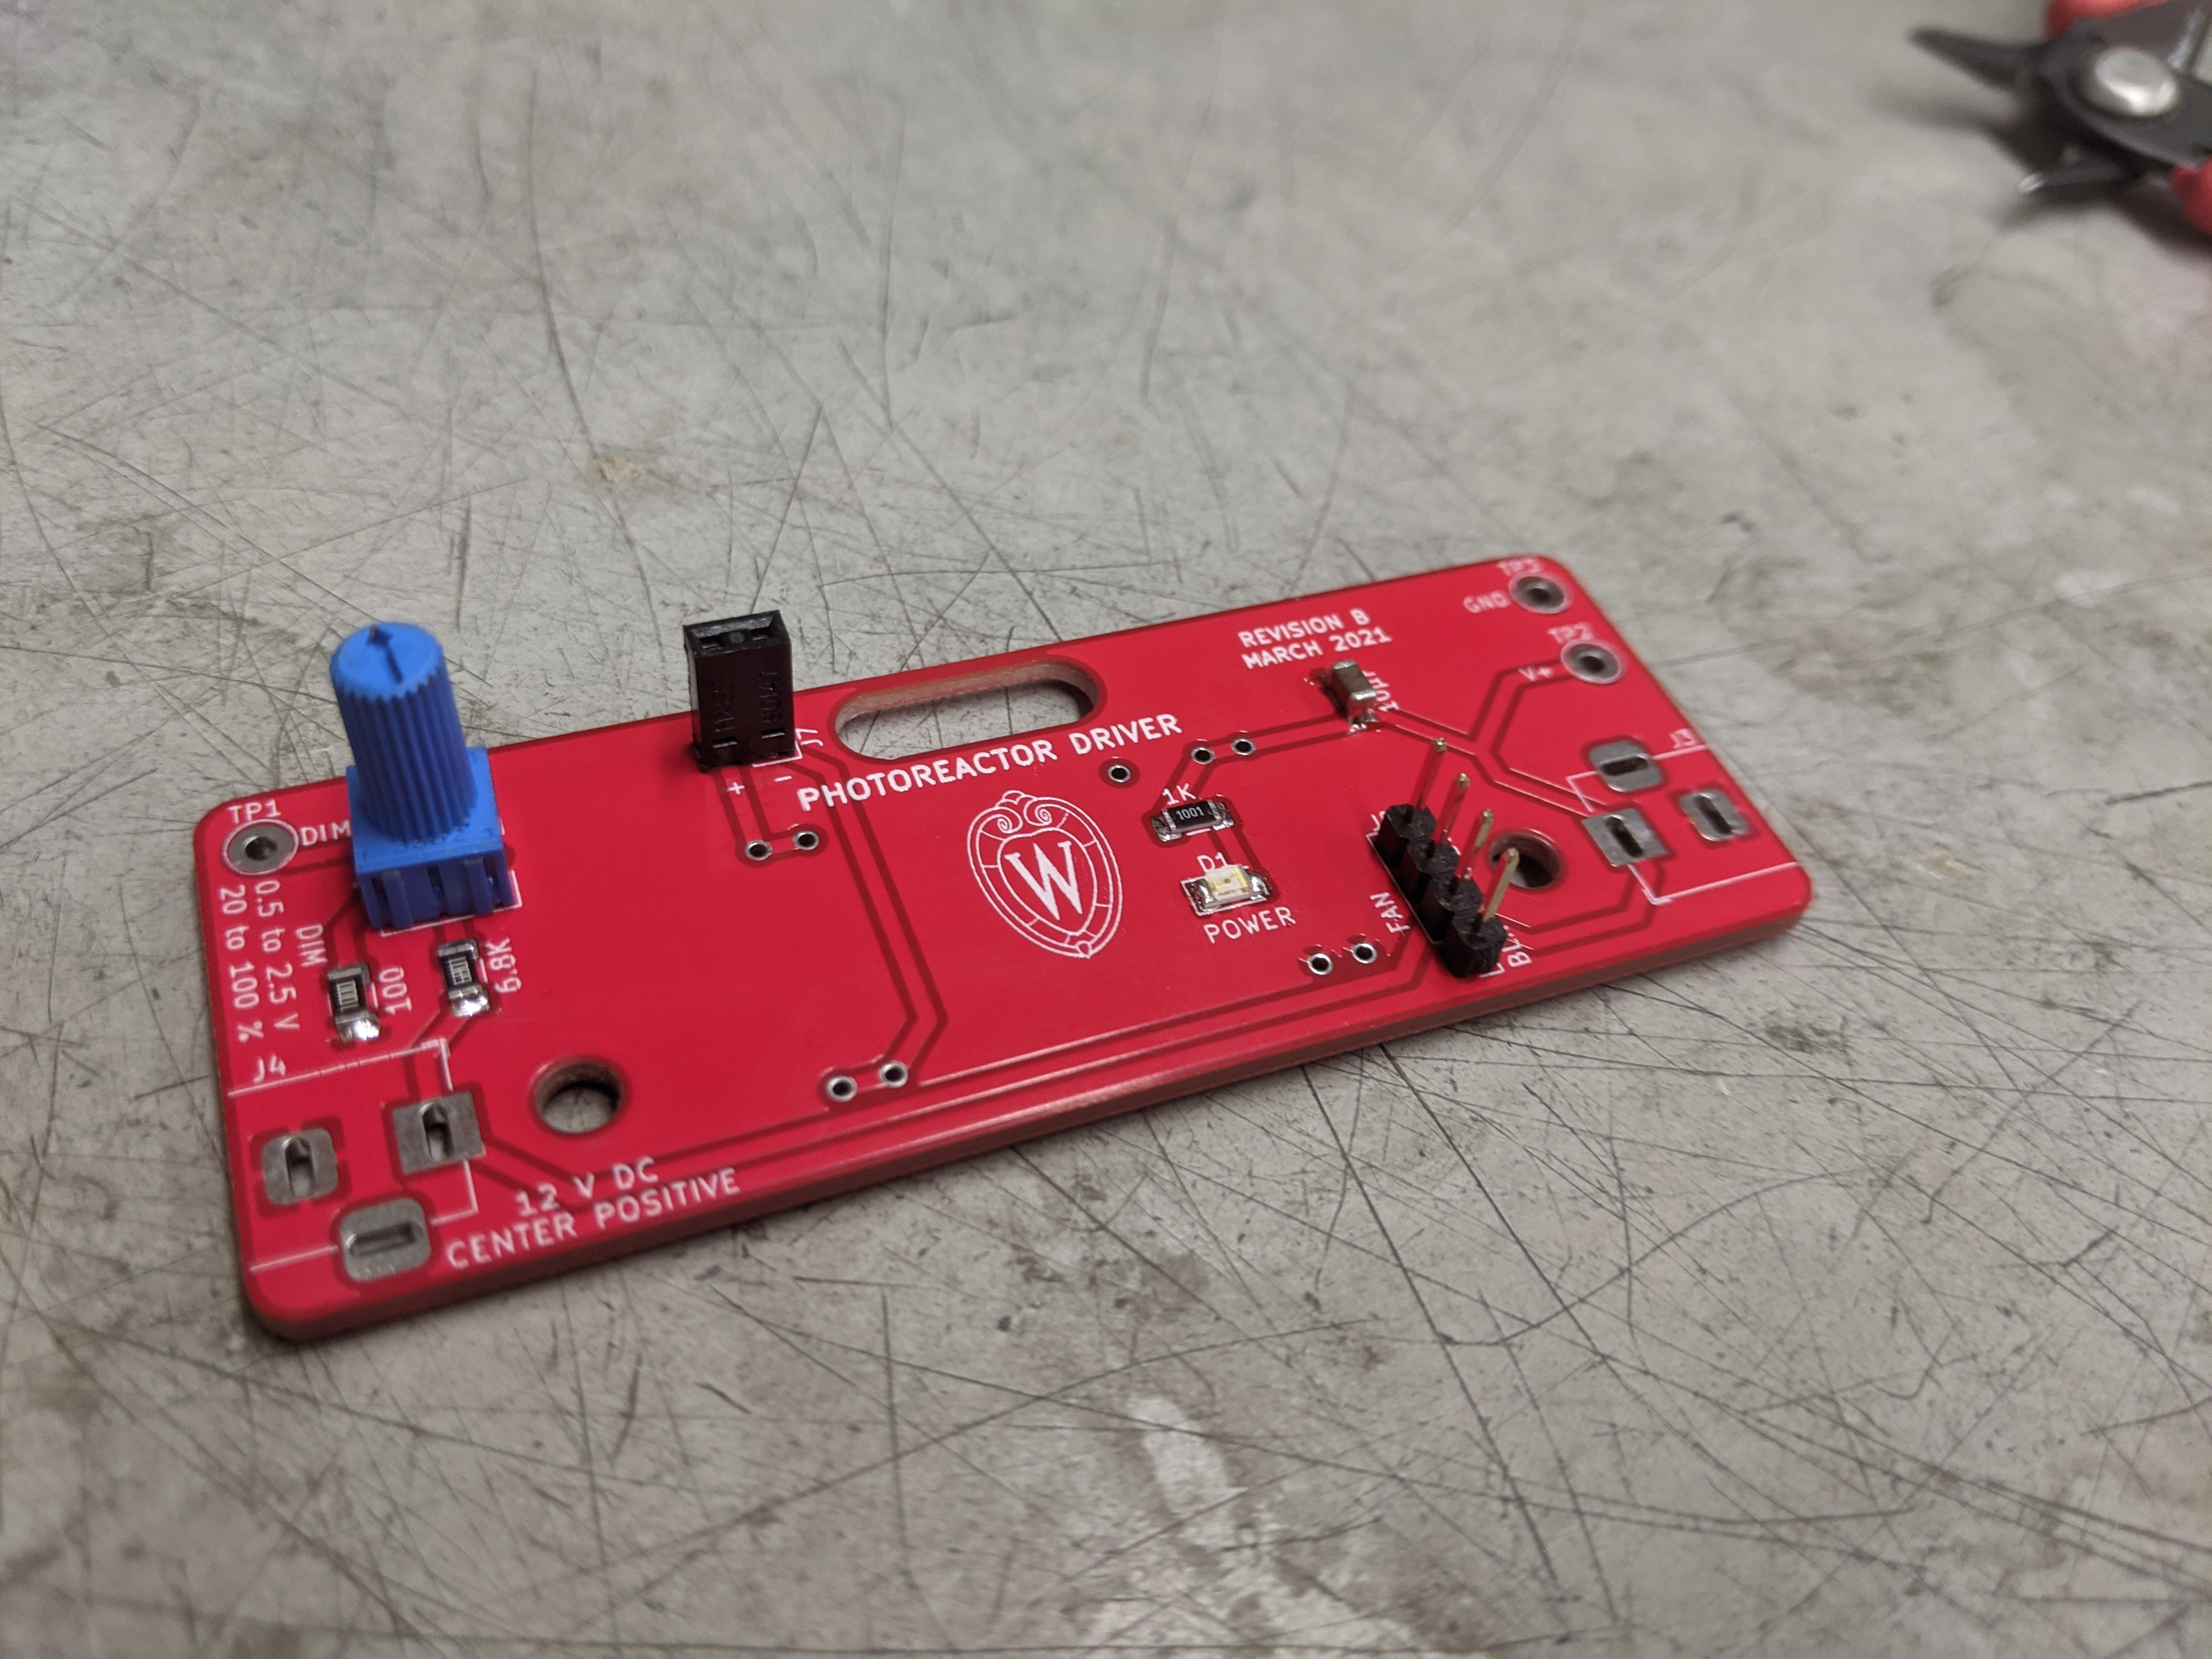
\includegraphics[width=\textwidth/2]{"./connectors.jpg"}
\end{center}

Next, add the connectors and the potentiometer knob.
From now on we recommend standard gage solder, e.g. 0.031''.
Once done your board should look like the above.

\begin{center}
  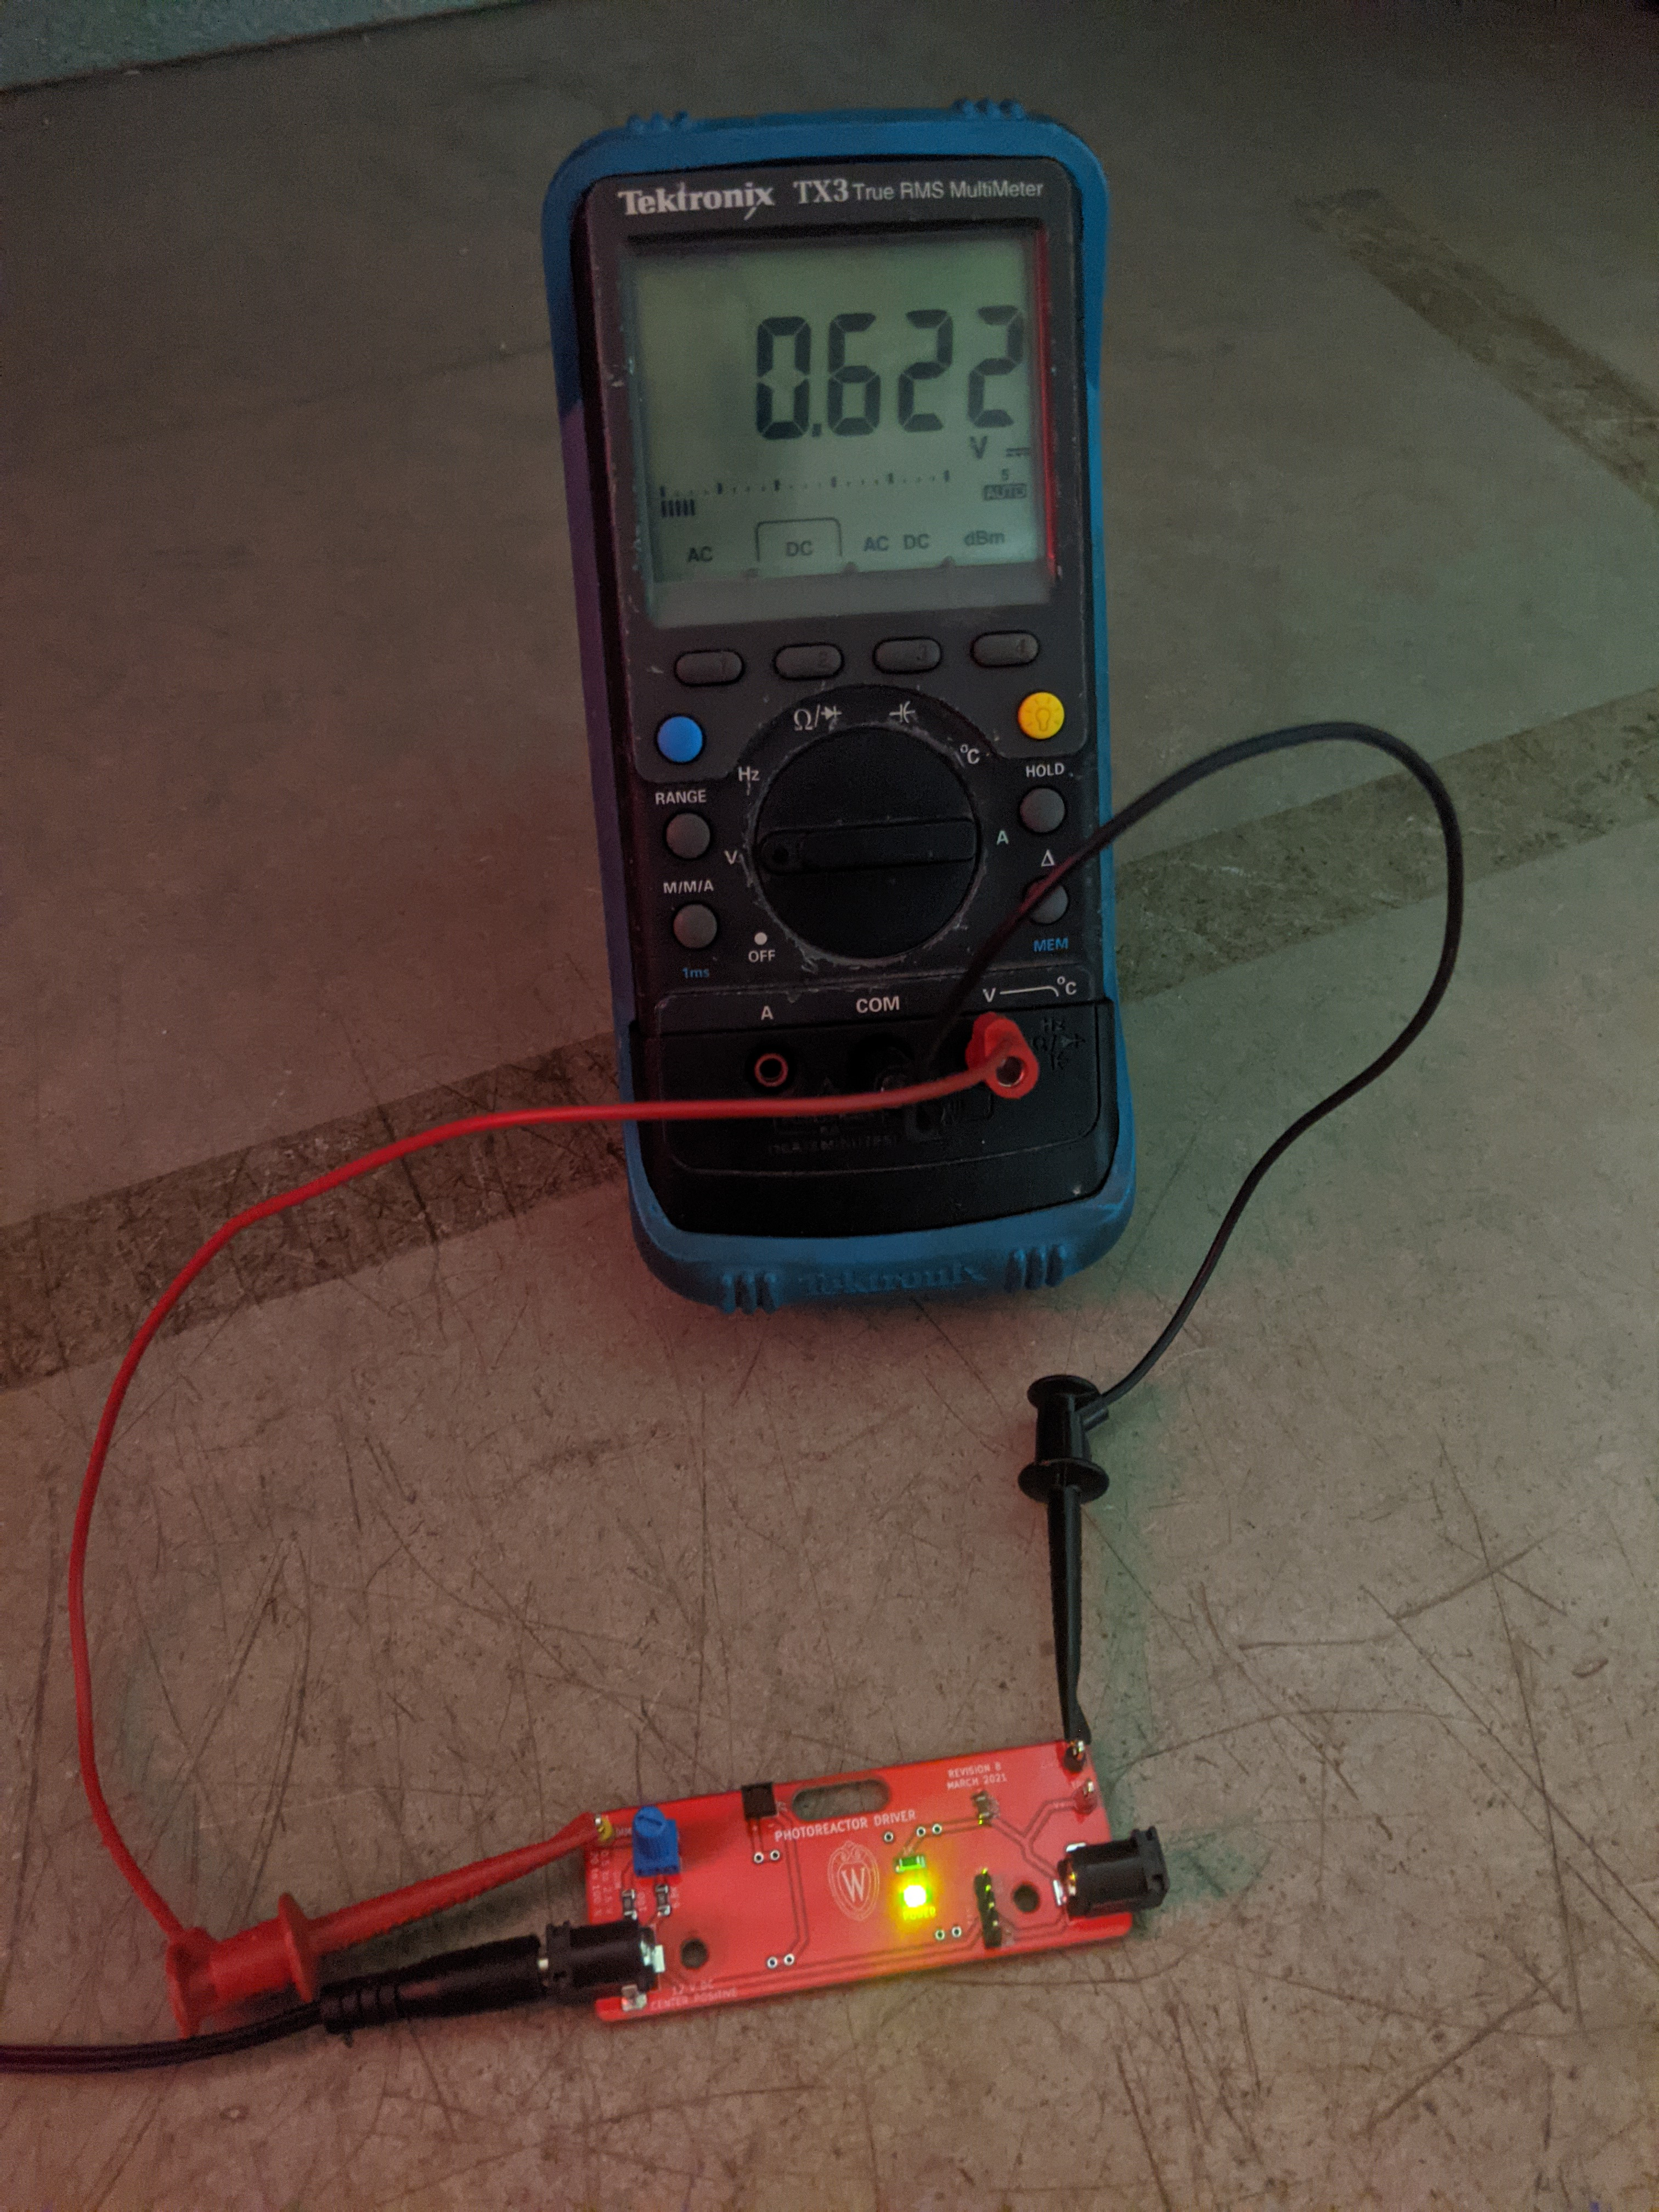
\includegraphics[width=\textwidth/2]{"./barrels-tested.jpg"}
\end{center}

Next, add the barrel jacks and the test points.
With these added you may plug in your board for the first time.
You should see your power indicator LED illuminate.
You should also be able to adjust the DC control voltage relative to ground by turning the knob, as shown above.

\begin{center}
  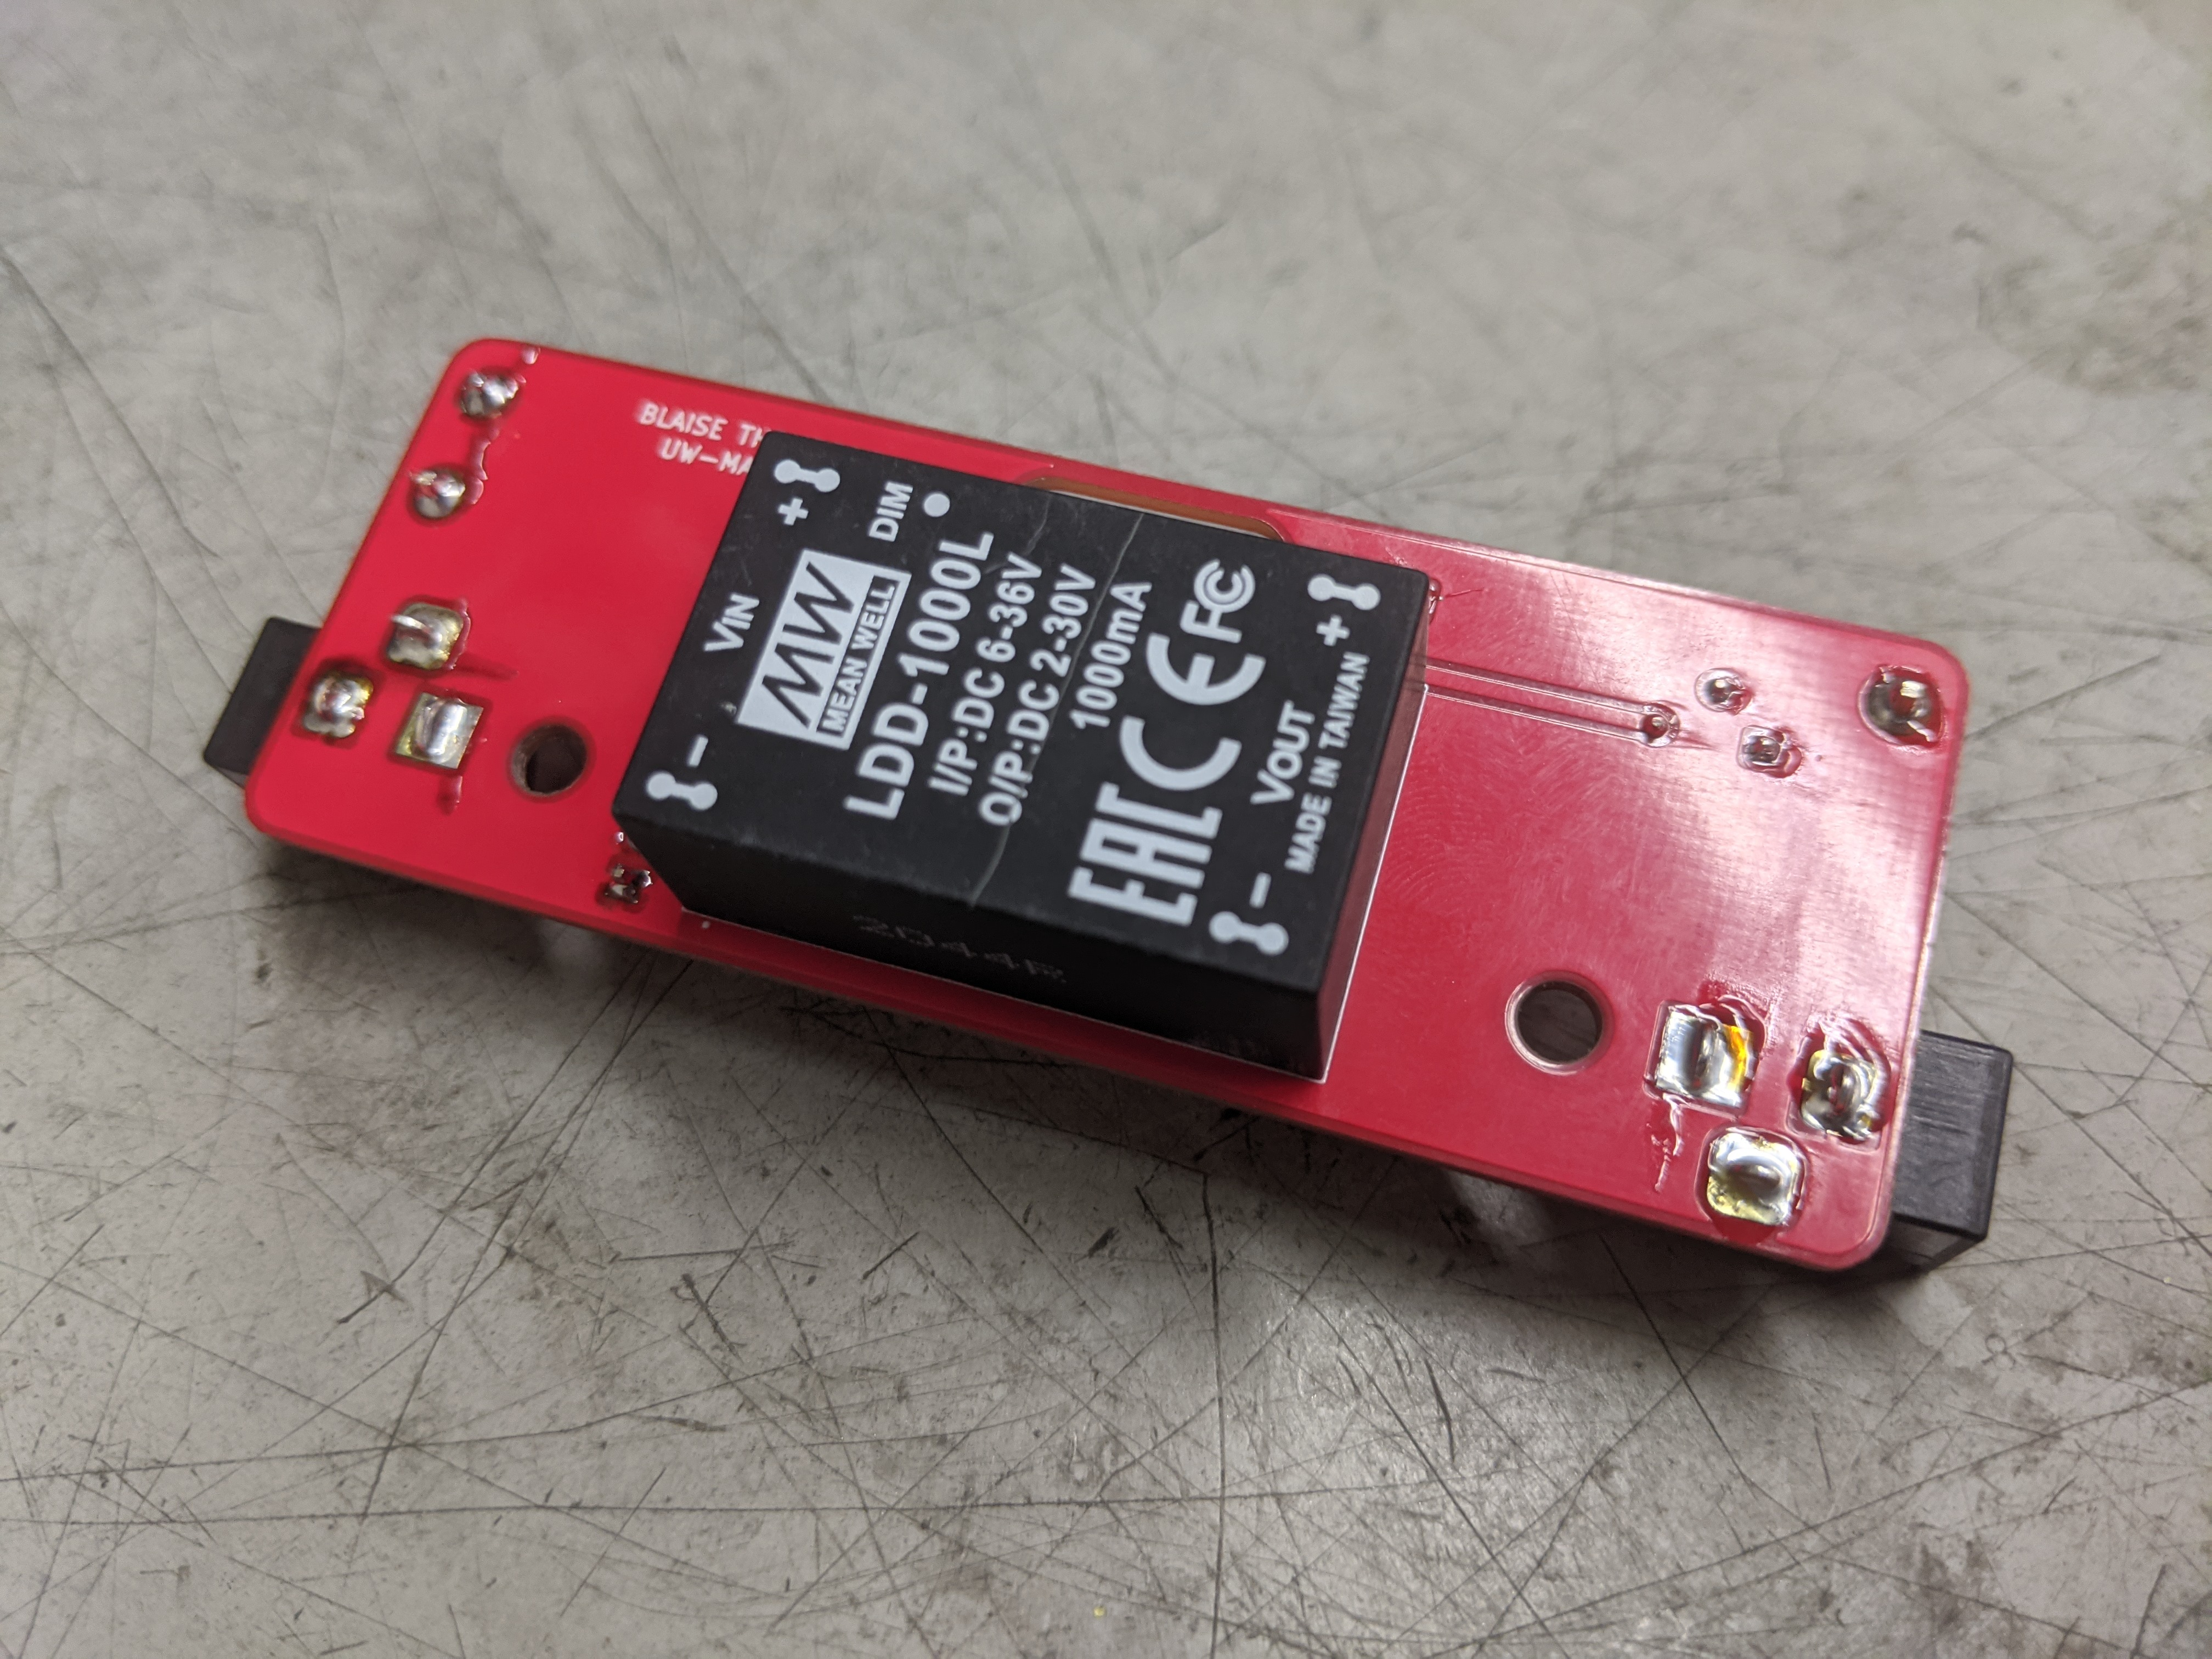
\includegraphics[width=\textwidth/2]{"./pcb-driver.jpg"}
\end{center}

Finally, add the Mean Well LED driver.
Note that this component goes on the back of the PCB, as shown above.

\includepdf[landscape=true]{"../analog-driver/driver.pdf"}

\subsection{Digital} \label{SEC:digital-driver}

The digital driver circuit can be controlled from a computer or some other digital device.
We built our driver to work over I2C, consistent with an emerging standard for many ``maker'' products.
While the physical connectors may be different, our digital circuit is compatible with the following systems.

\begin{itemize}
  \item \href{https://learn.adafruit.com/introducing-adafruit-stemma-qt}{Adafruit STEMMA}
  \item \href{https://www.sparkfun.com/qwiic}{Sparkfun Qwiic}
  \item \href{https://www.seeedstudio.com/category/Grove-c-1003.html}{Seeed Grove}
\end{itemize}

\begin{center}
  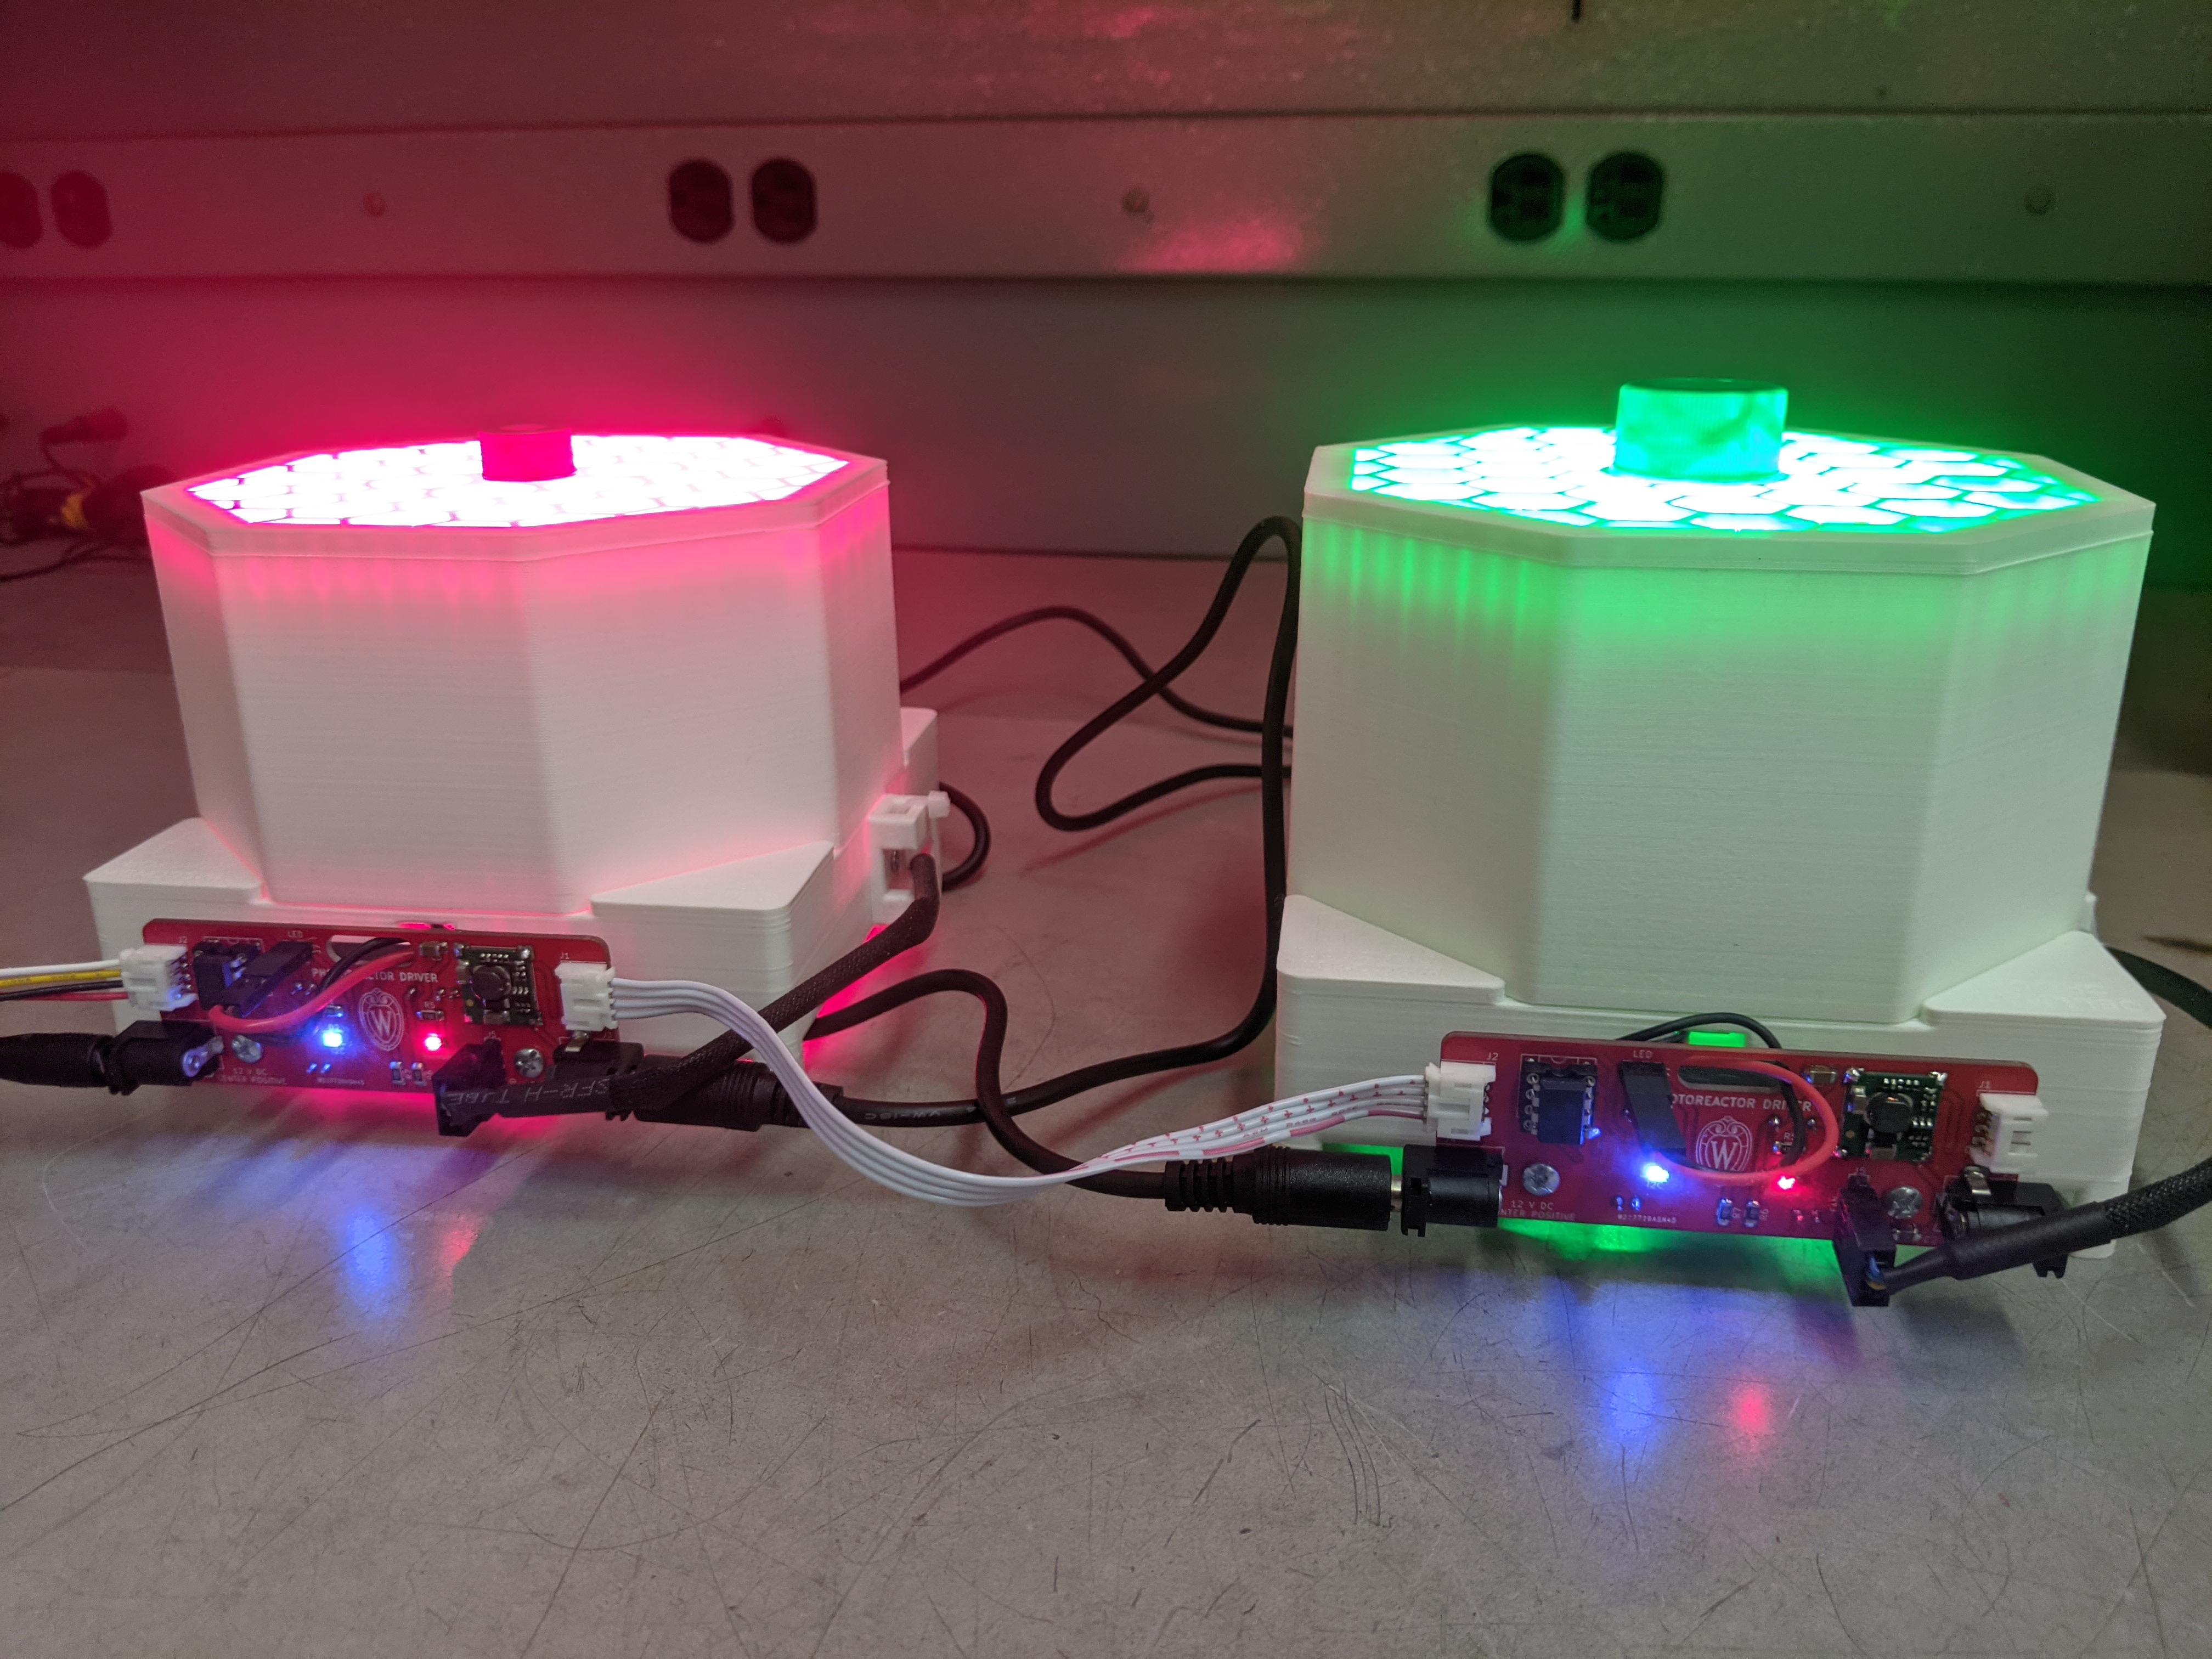
\includegraphics[width=\textwidth/2]{"./digital-wired.jpg"}
\end{center}

Each digital driver is based around an ATtiny85 microcontroller acting as an I2C peripheral.
Multiple digital driver boards may be ``networked'' together onto one I2C bus by simply daisy-chaining the boards together, as shown above.
In such a use-case you must choose a unique I2C address for each ATtiny85 peripheral.

\begin{center}
  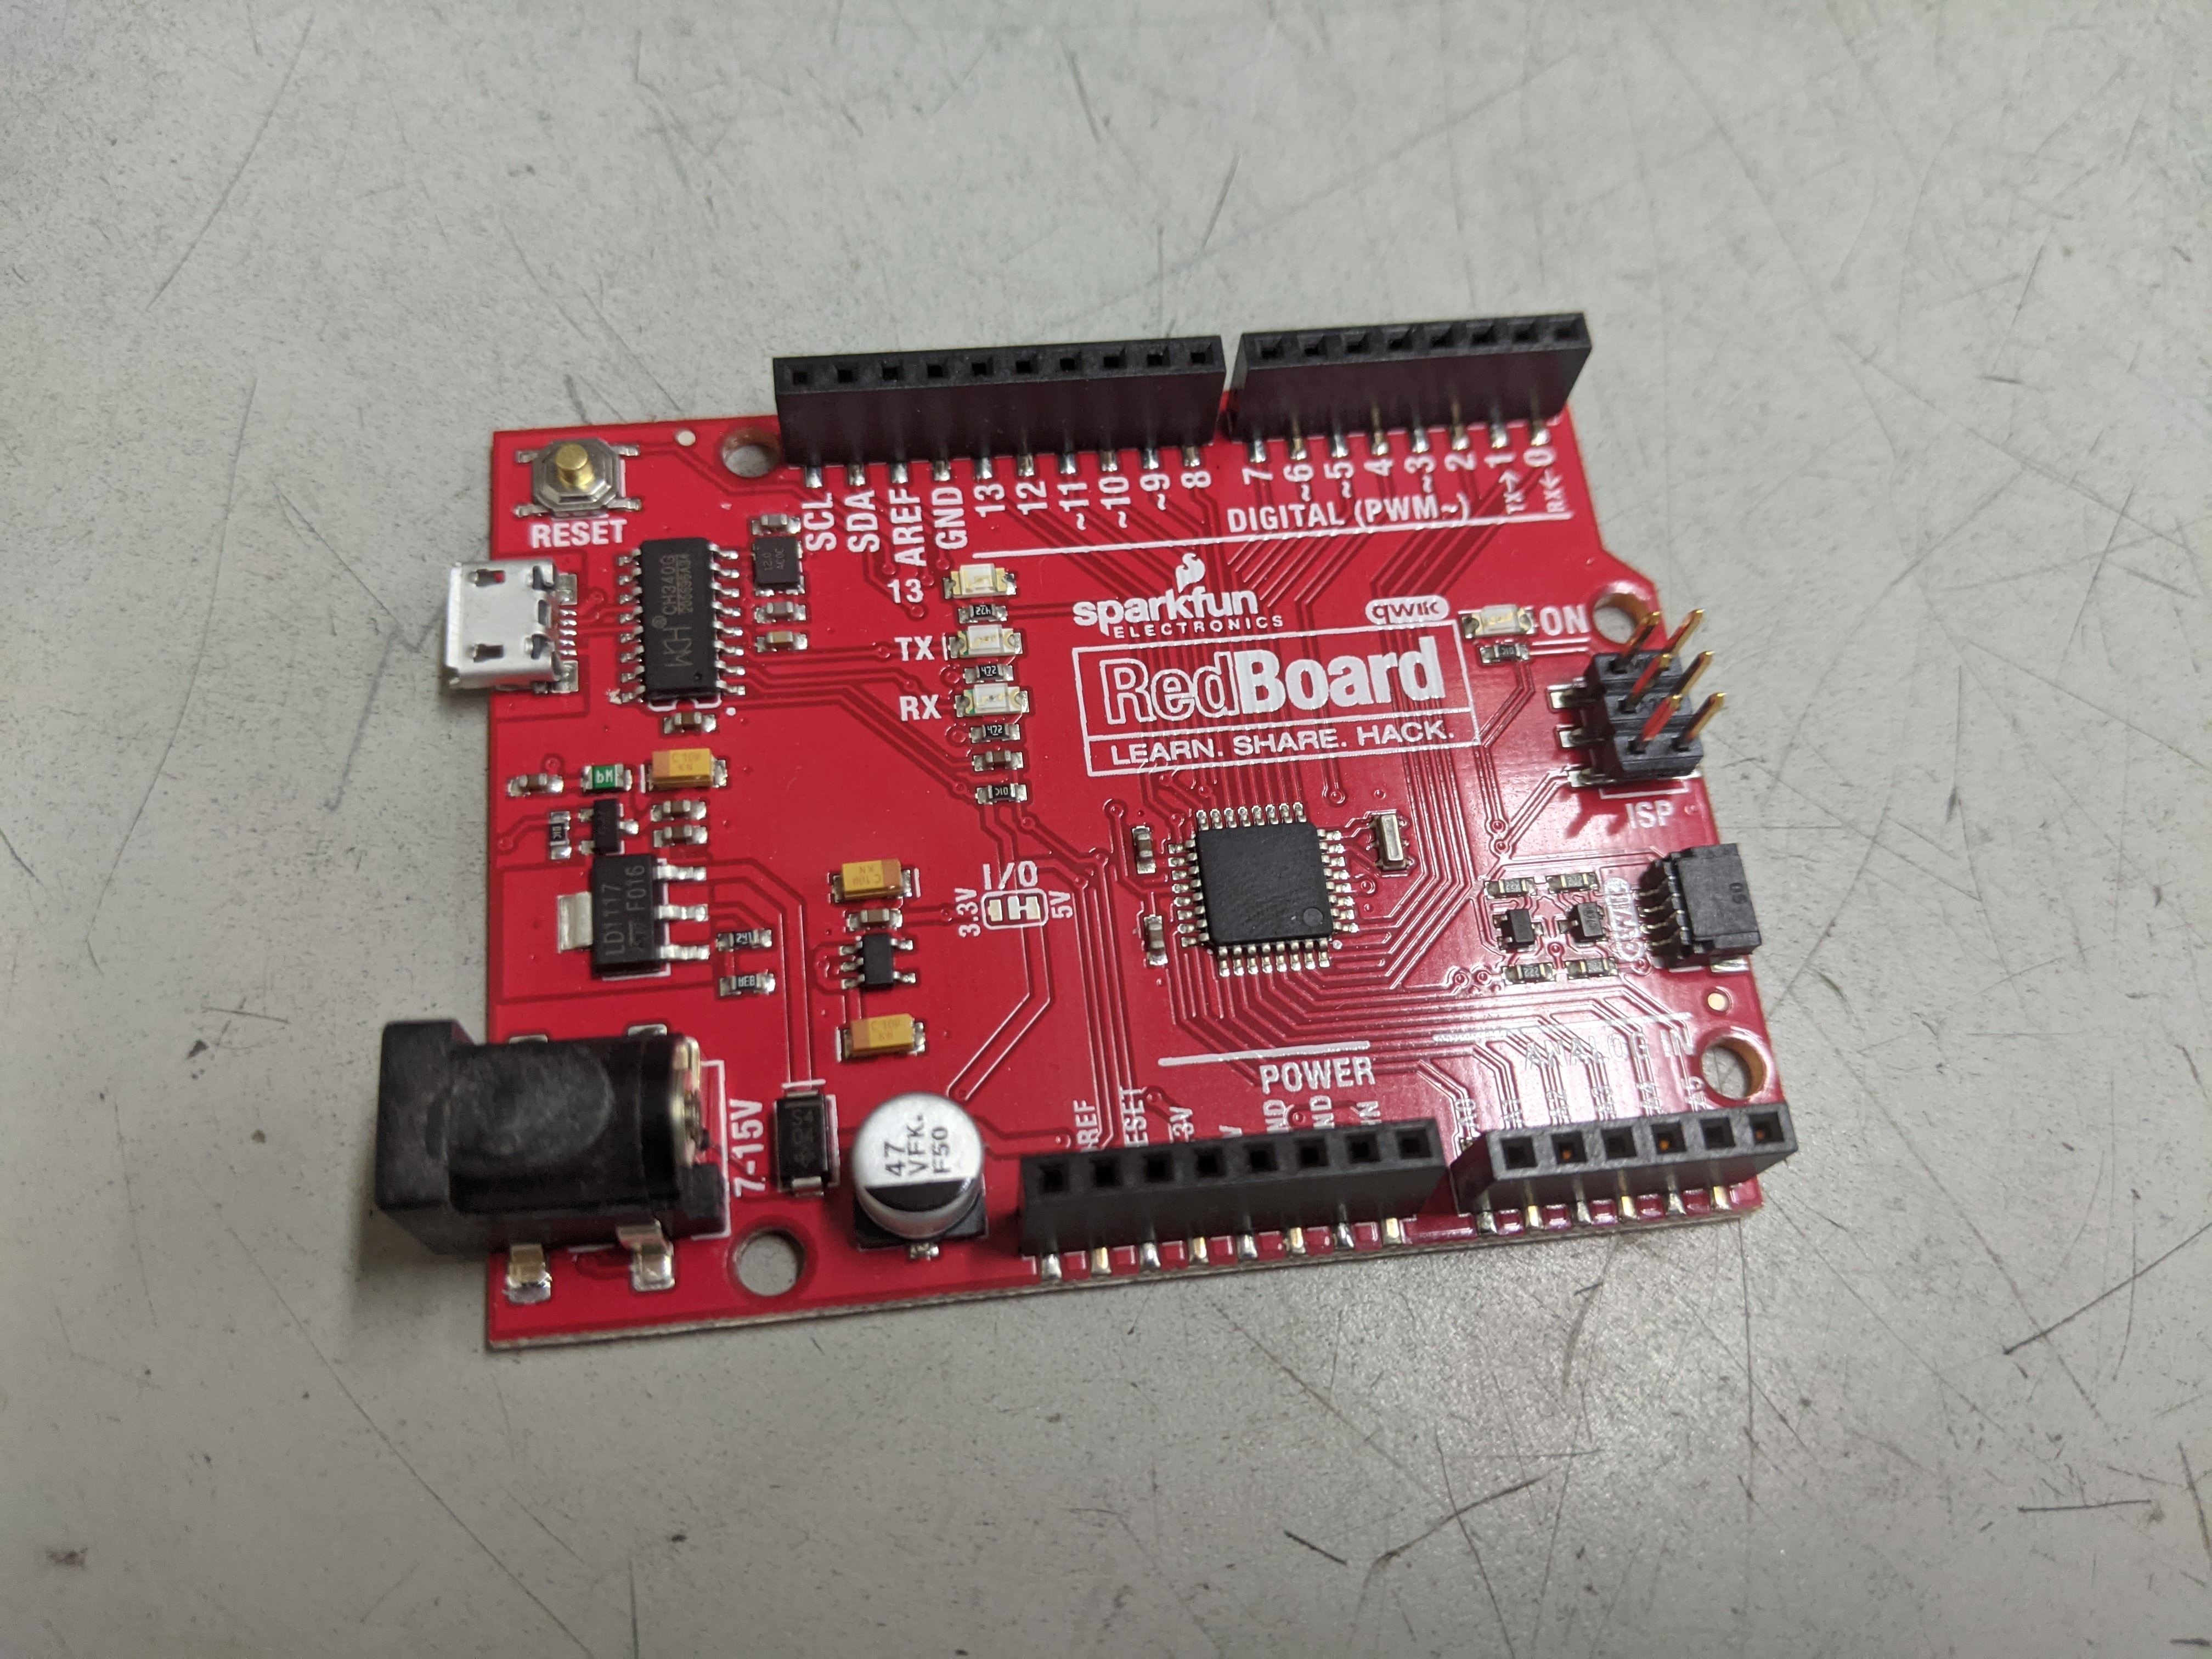
\includegraphics[width=\textwidth/2]{"./redboard.jpg"}
\end{center}

There are many ways to interface with the I2C bus.
We have used a SparkFun RedBoard, pictured above.
You may find an example within the online repository that dynamically controls both the LED intensity and fan speed.

\includepdf[landscape=true]{"../digital-driver/driver.pdf"}

\section{Assembly} \label{SEC:assembly}

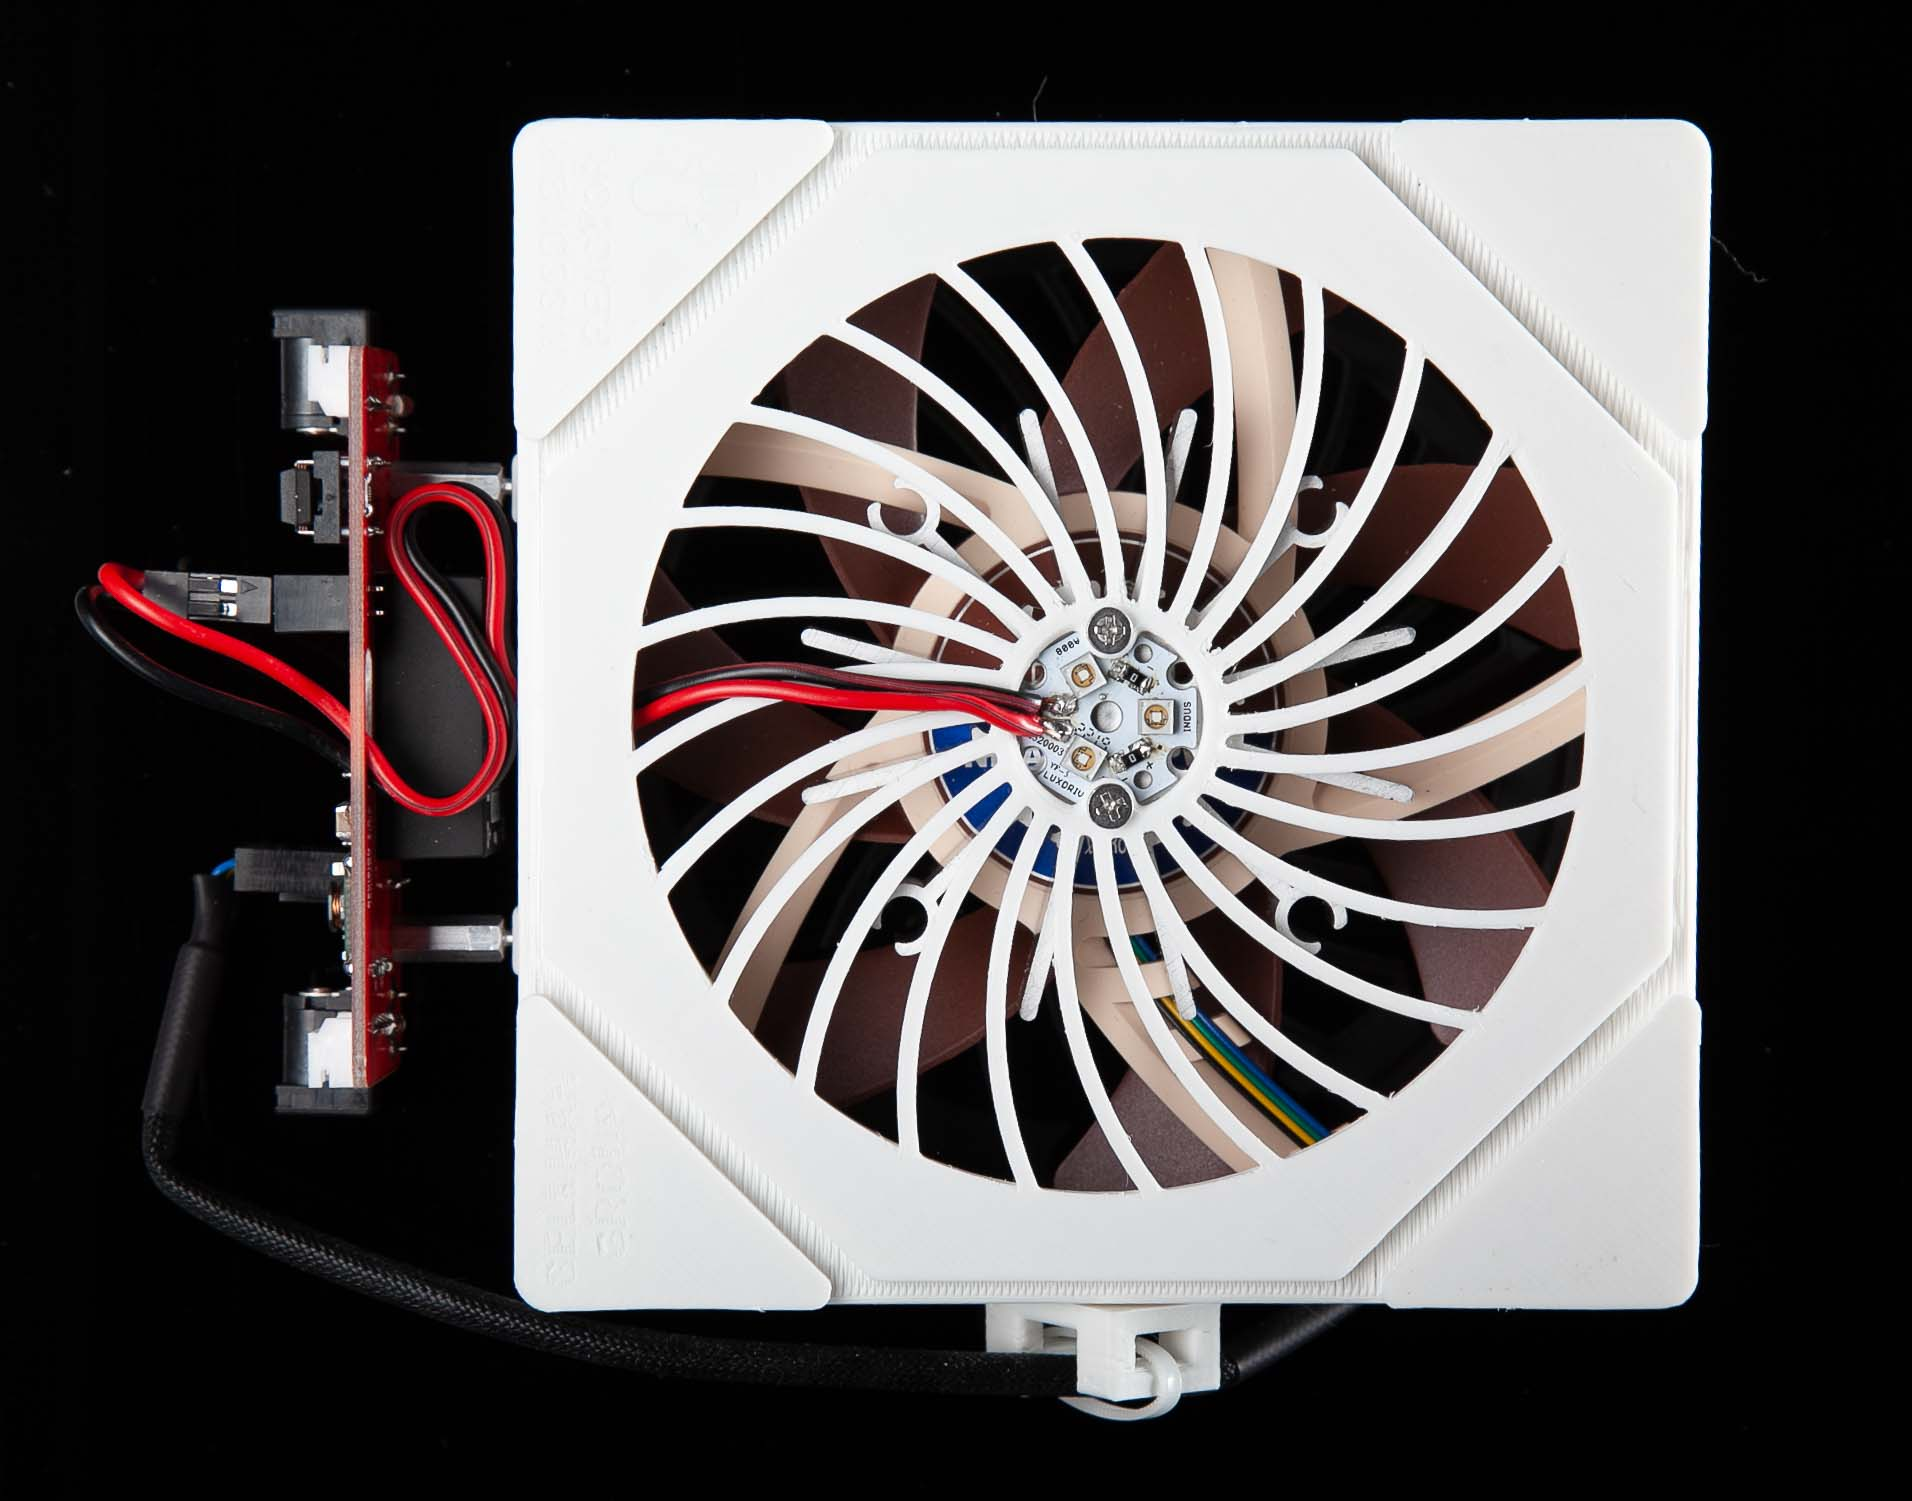
\includegraphics[width=\textwidth]{"./assembly-coverart.jpg"}

Once 3D printing is done and PCBs have been filled, WPR assembly is fairly straight-forward.
The various electronic components must be installed into the base (pictured above), as described in \autoref{SEC:base}.
Reflective coating must be added to the chamber walls, as described in \autoref{SEC:top}.
After these final steps, your WPR is ready for synthesis!

\clearpage
\subsection{Base} \label{SEC:base}

\begin{center}
  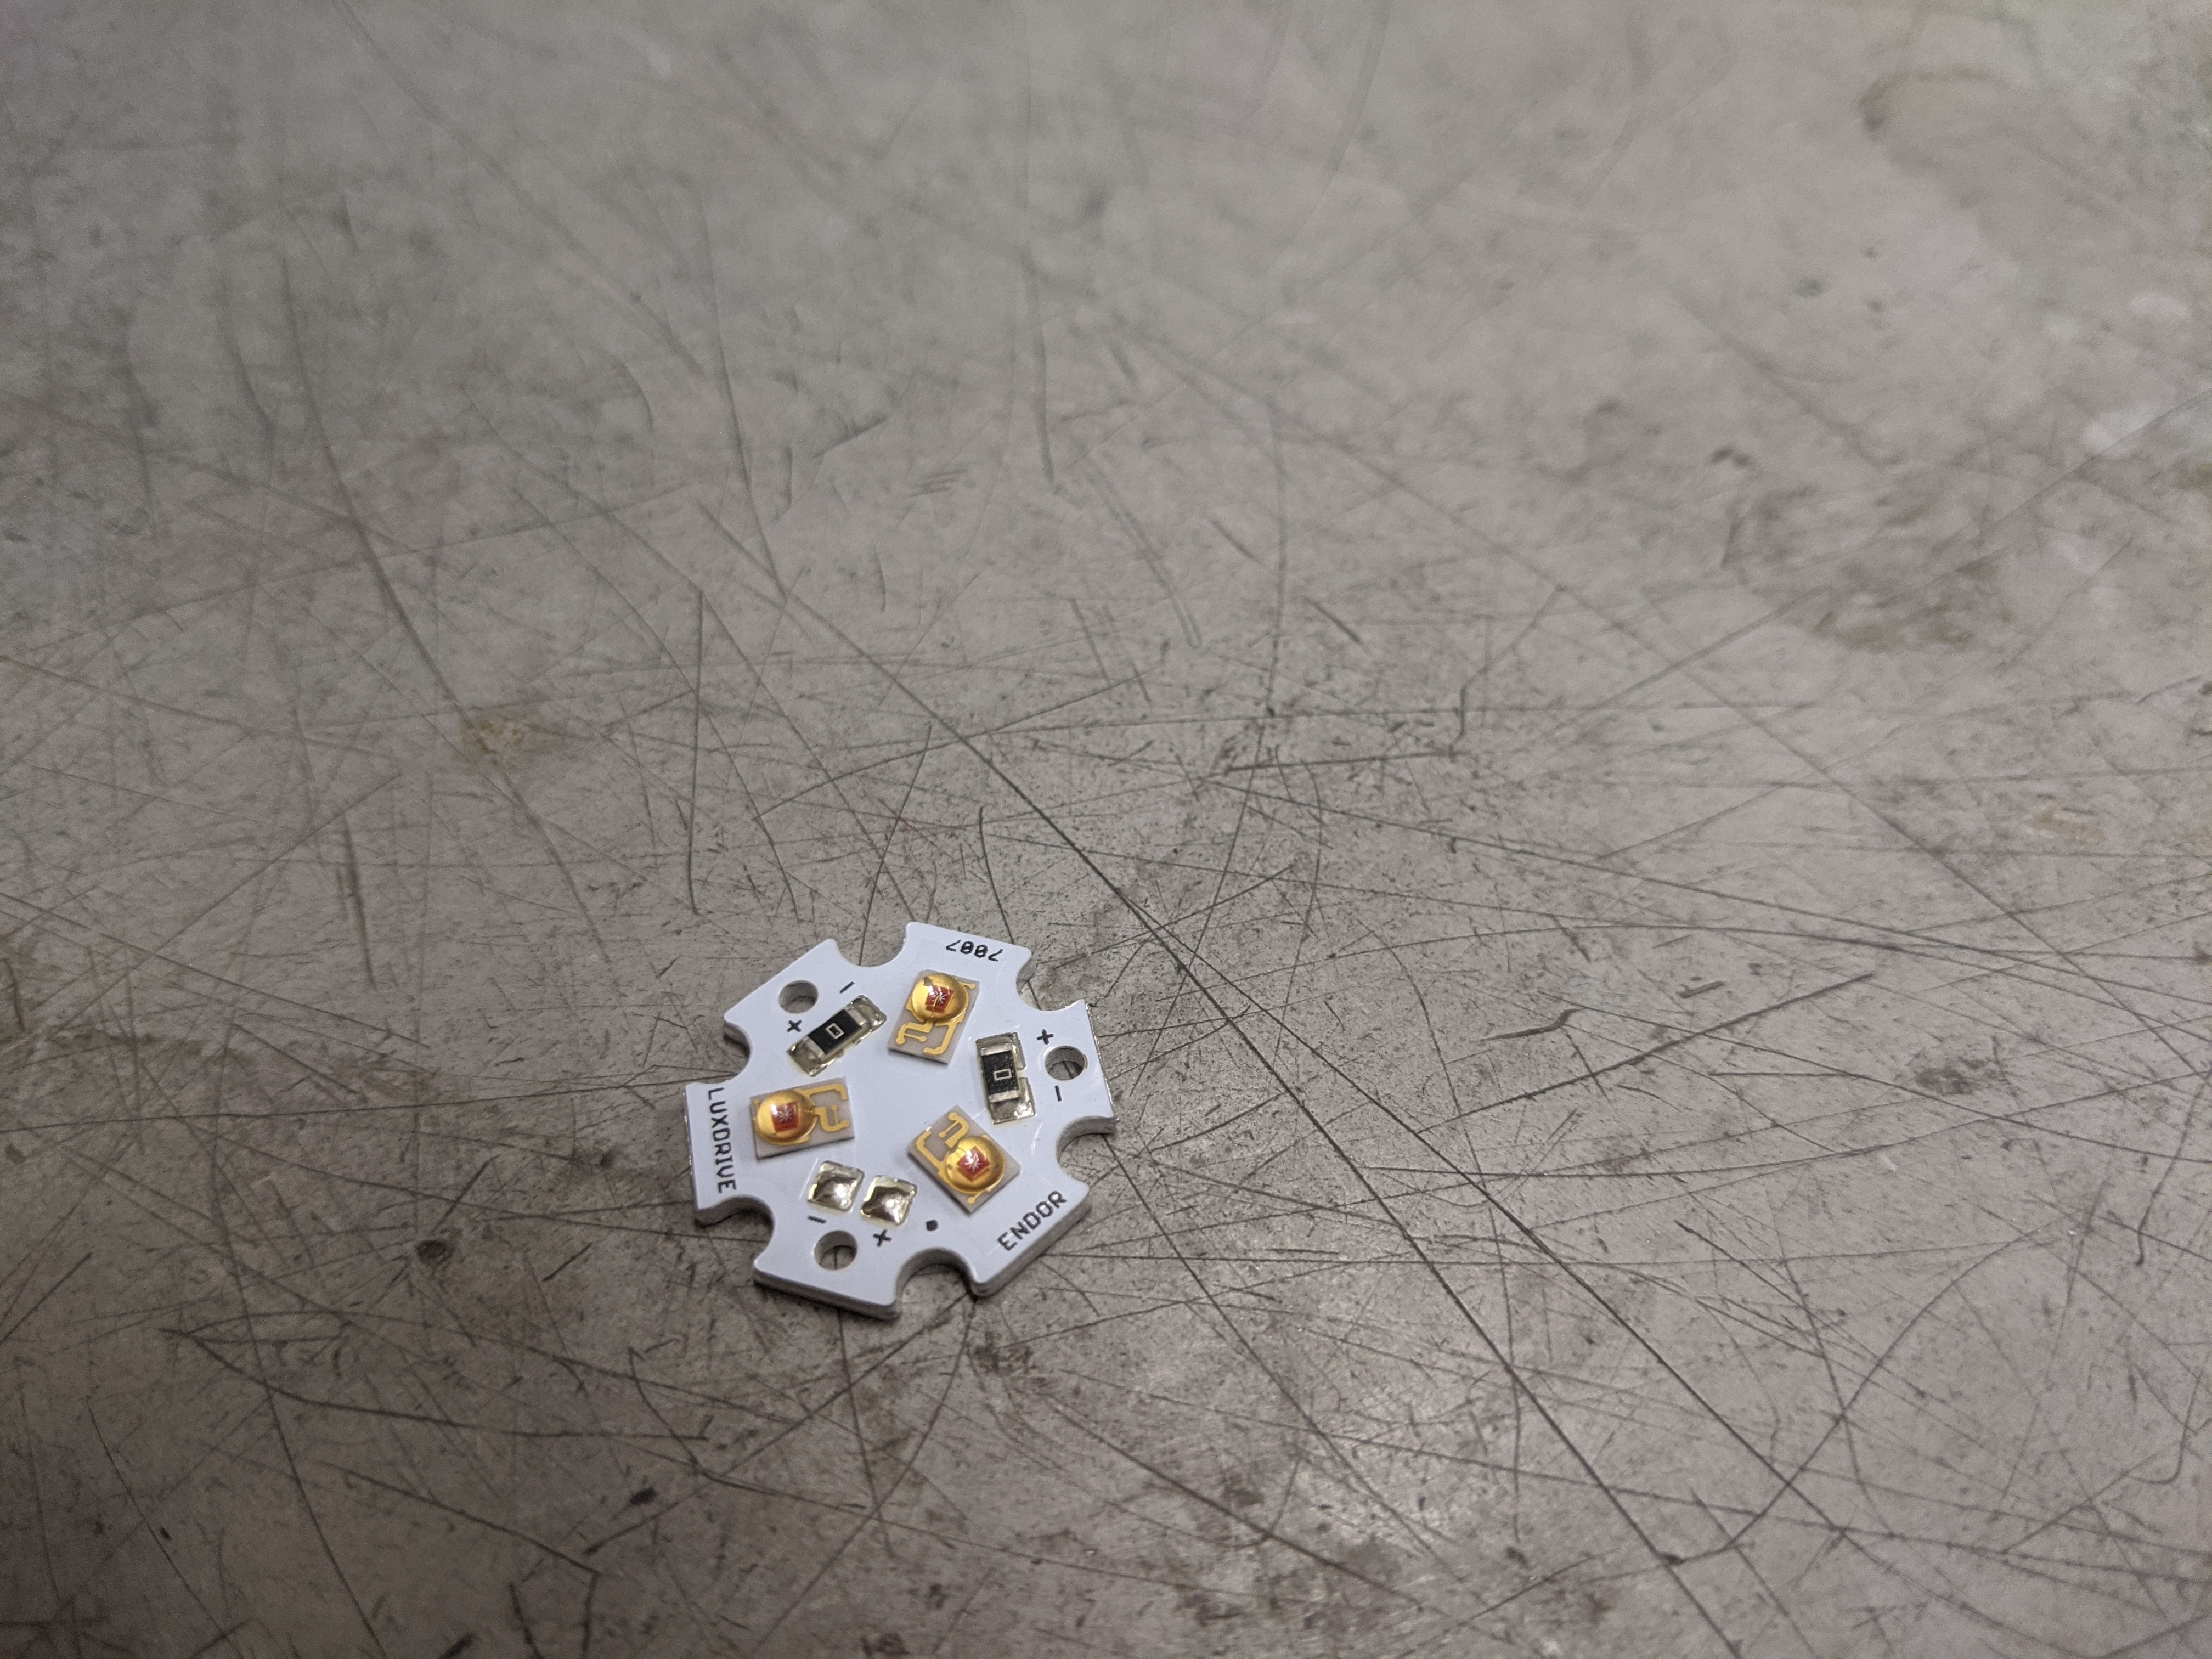
\includegraphics[width=\textwidth/2]{"./bare-led.jpg"}
\end{center}

If possible, it's best to order your LEDs pre-attached to an ``LED star'' heat sink.
Otherwise you may order bare LED stars and discrete LEDs.
Either way, you will have a filled LED star as pictured above.
In this example we are using LED Supply part number 07007-PL000-F.

\begin{center}
  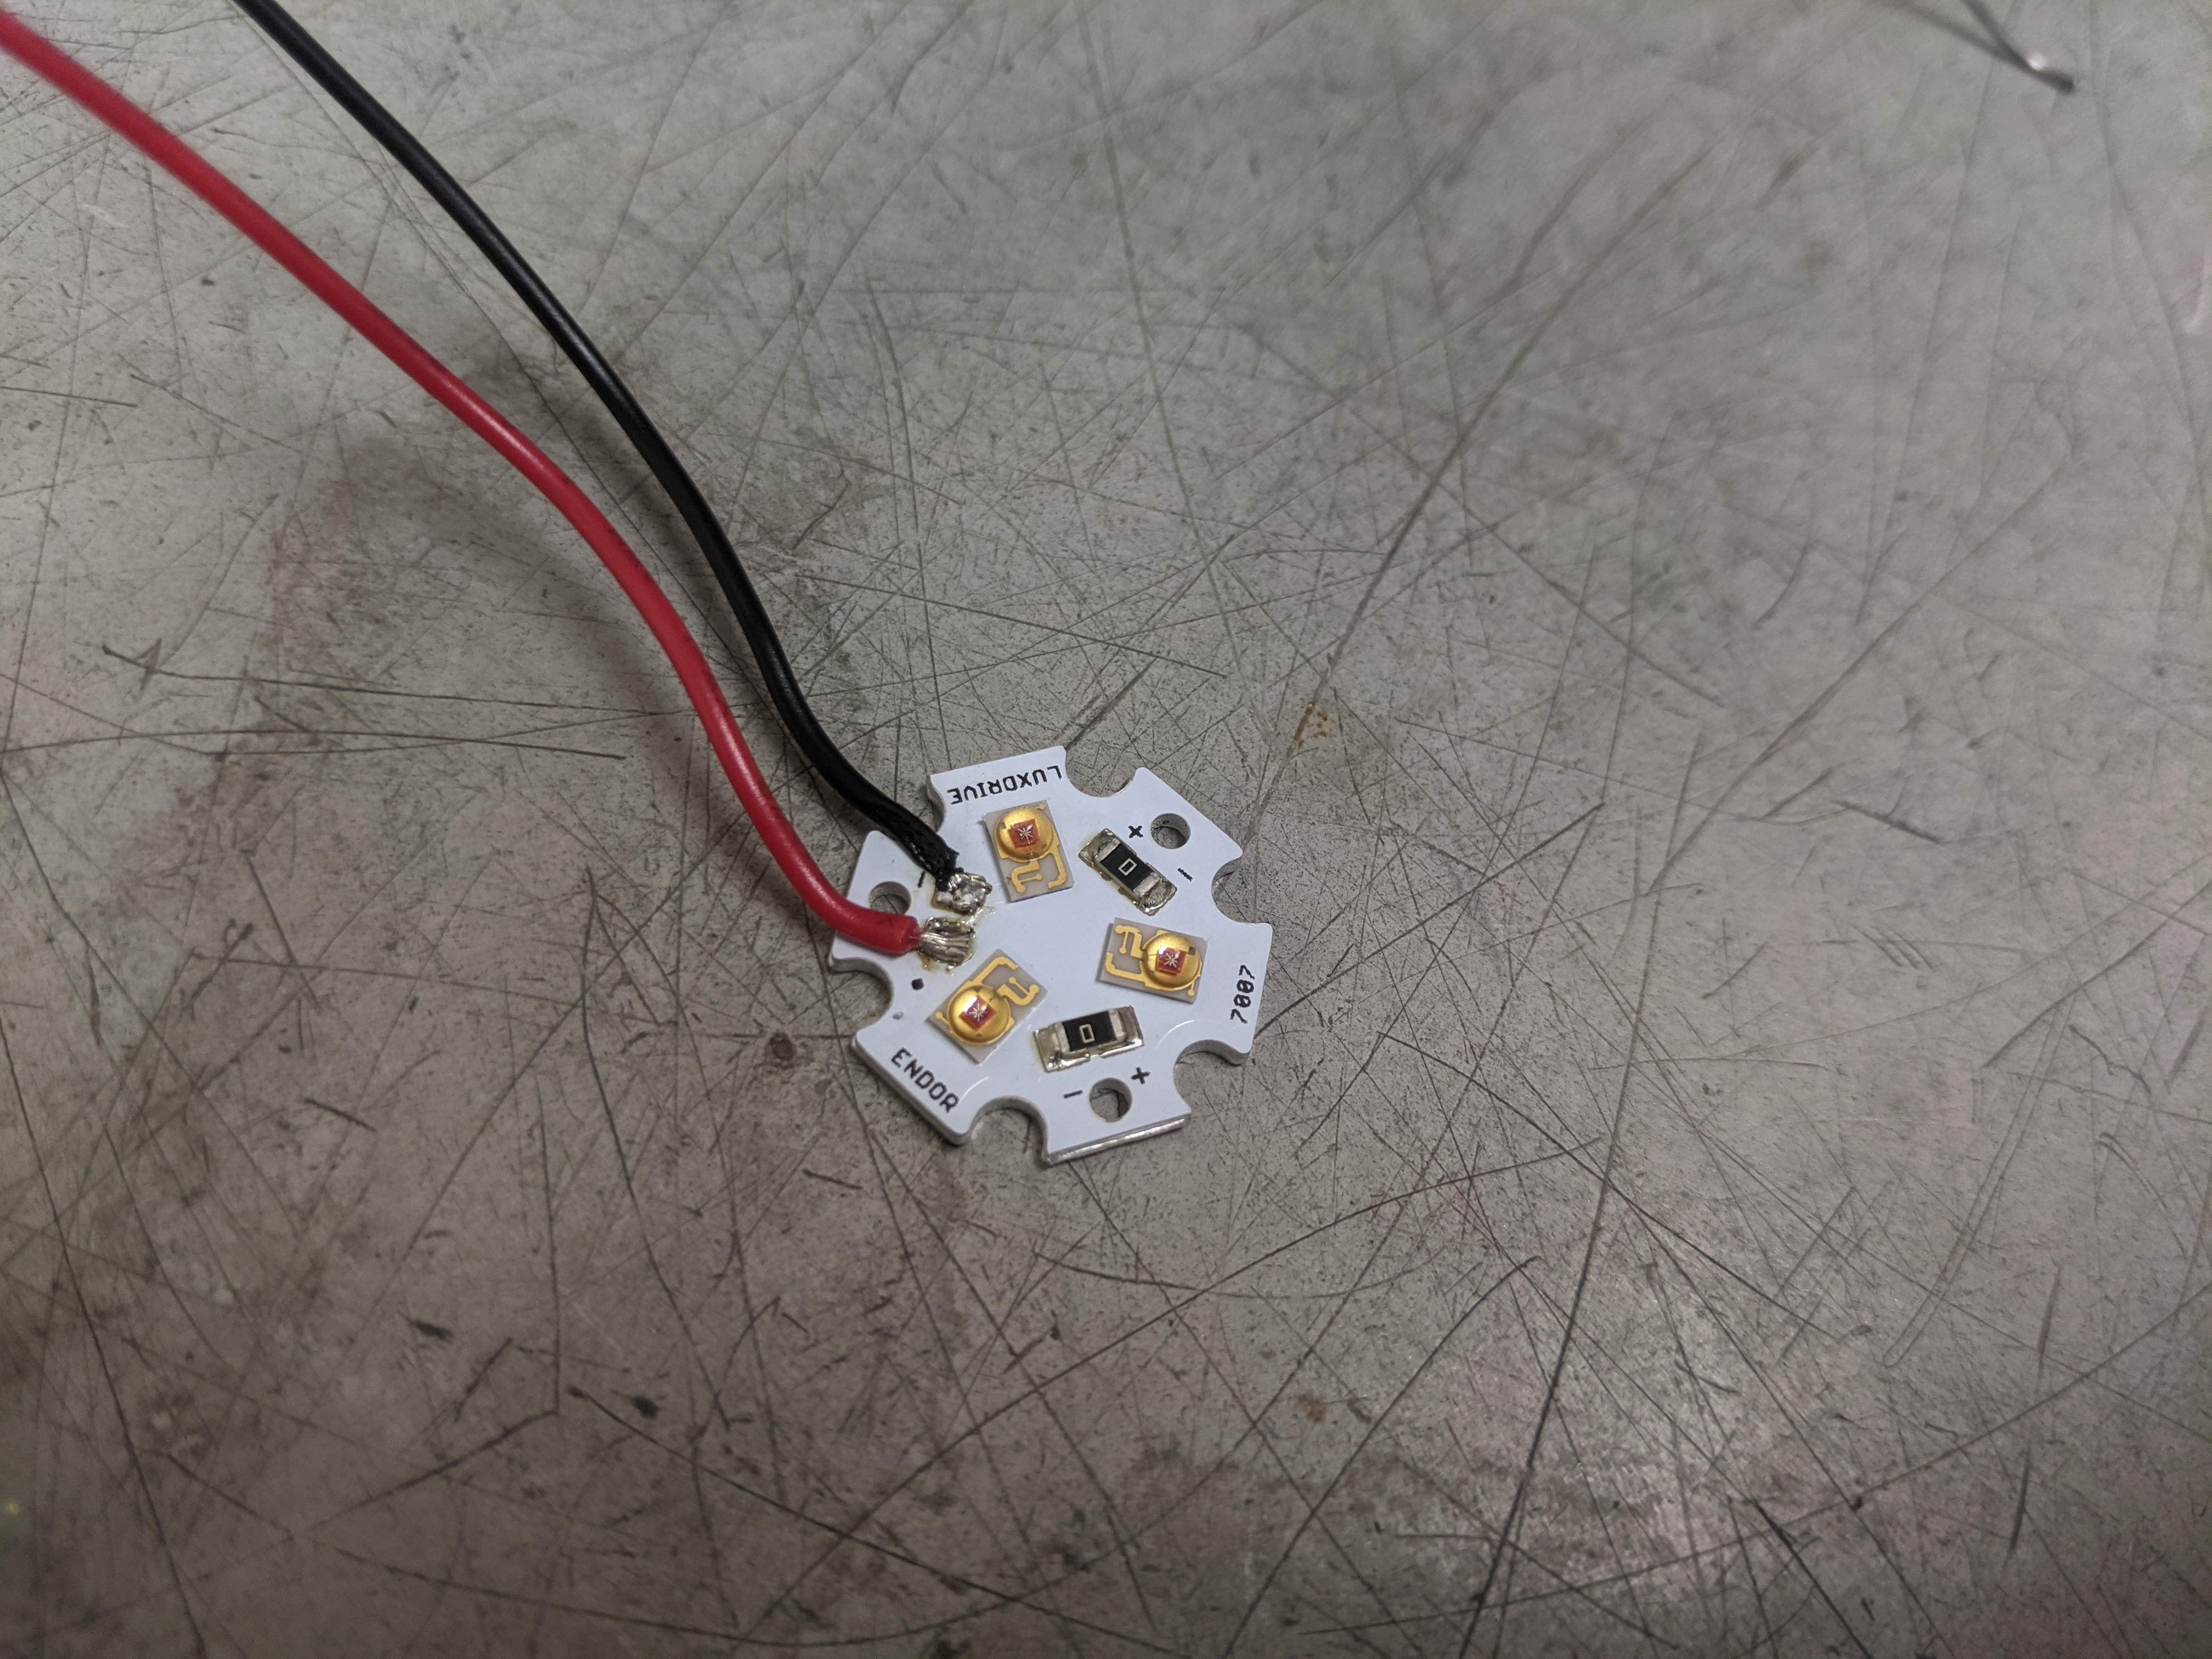
\includegraphics[width=\textwidth/2]{"./soldered-led.jpg"}
\end{center}

Start by soldering leads onto your LED star, using the red positive black negative convention.
Soldering here may be challenging, as the LED star itself will resist your efforts to heat it.
Adding some lead-based solder may help, due to the lower melting point.

\begin{center}
  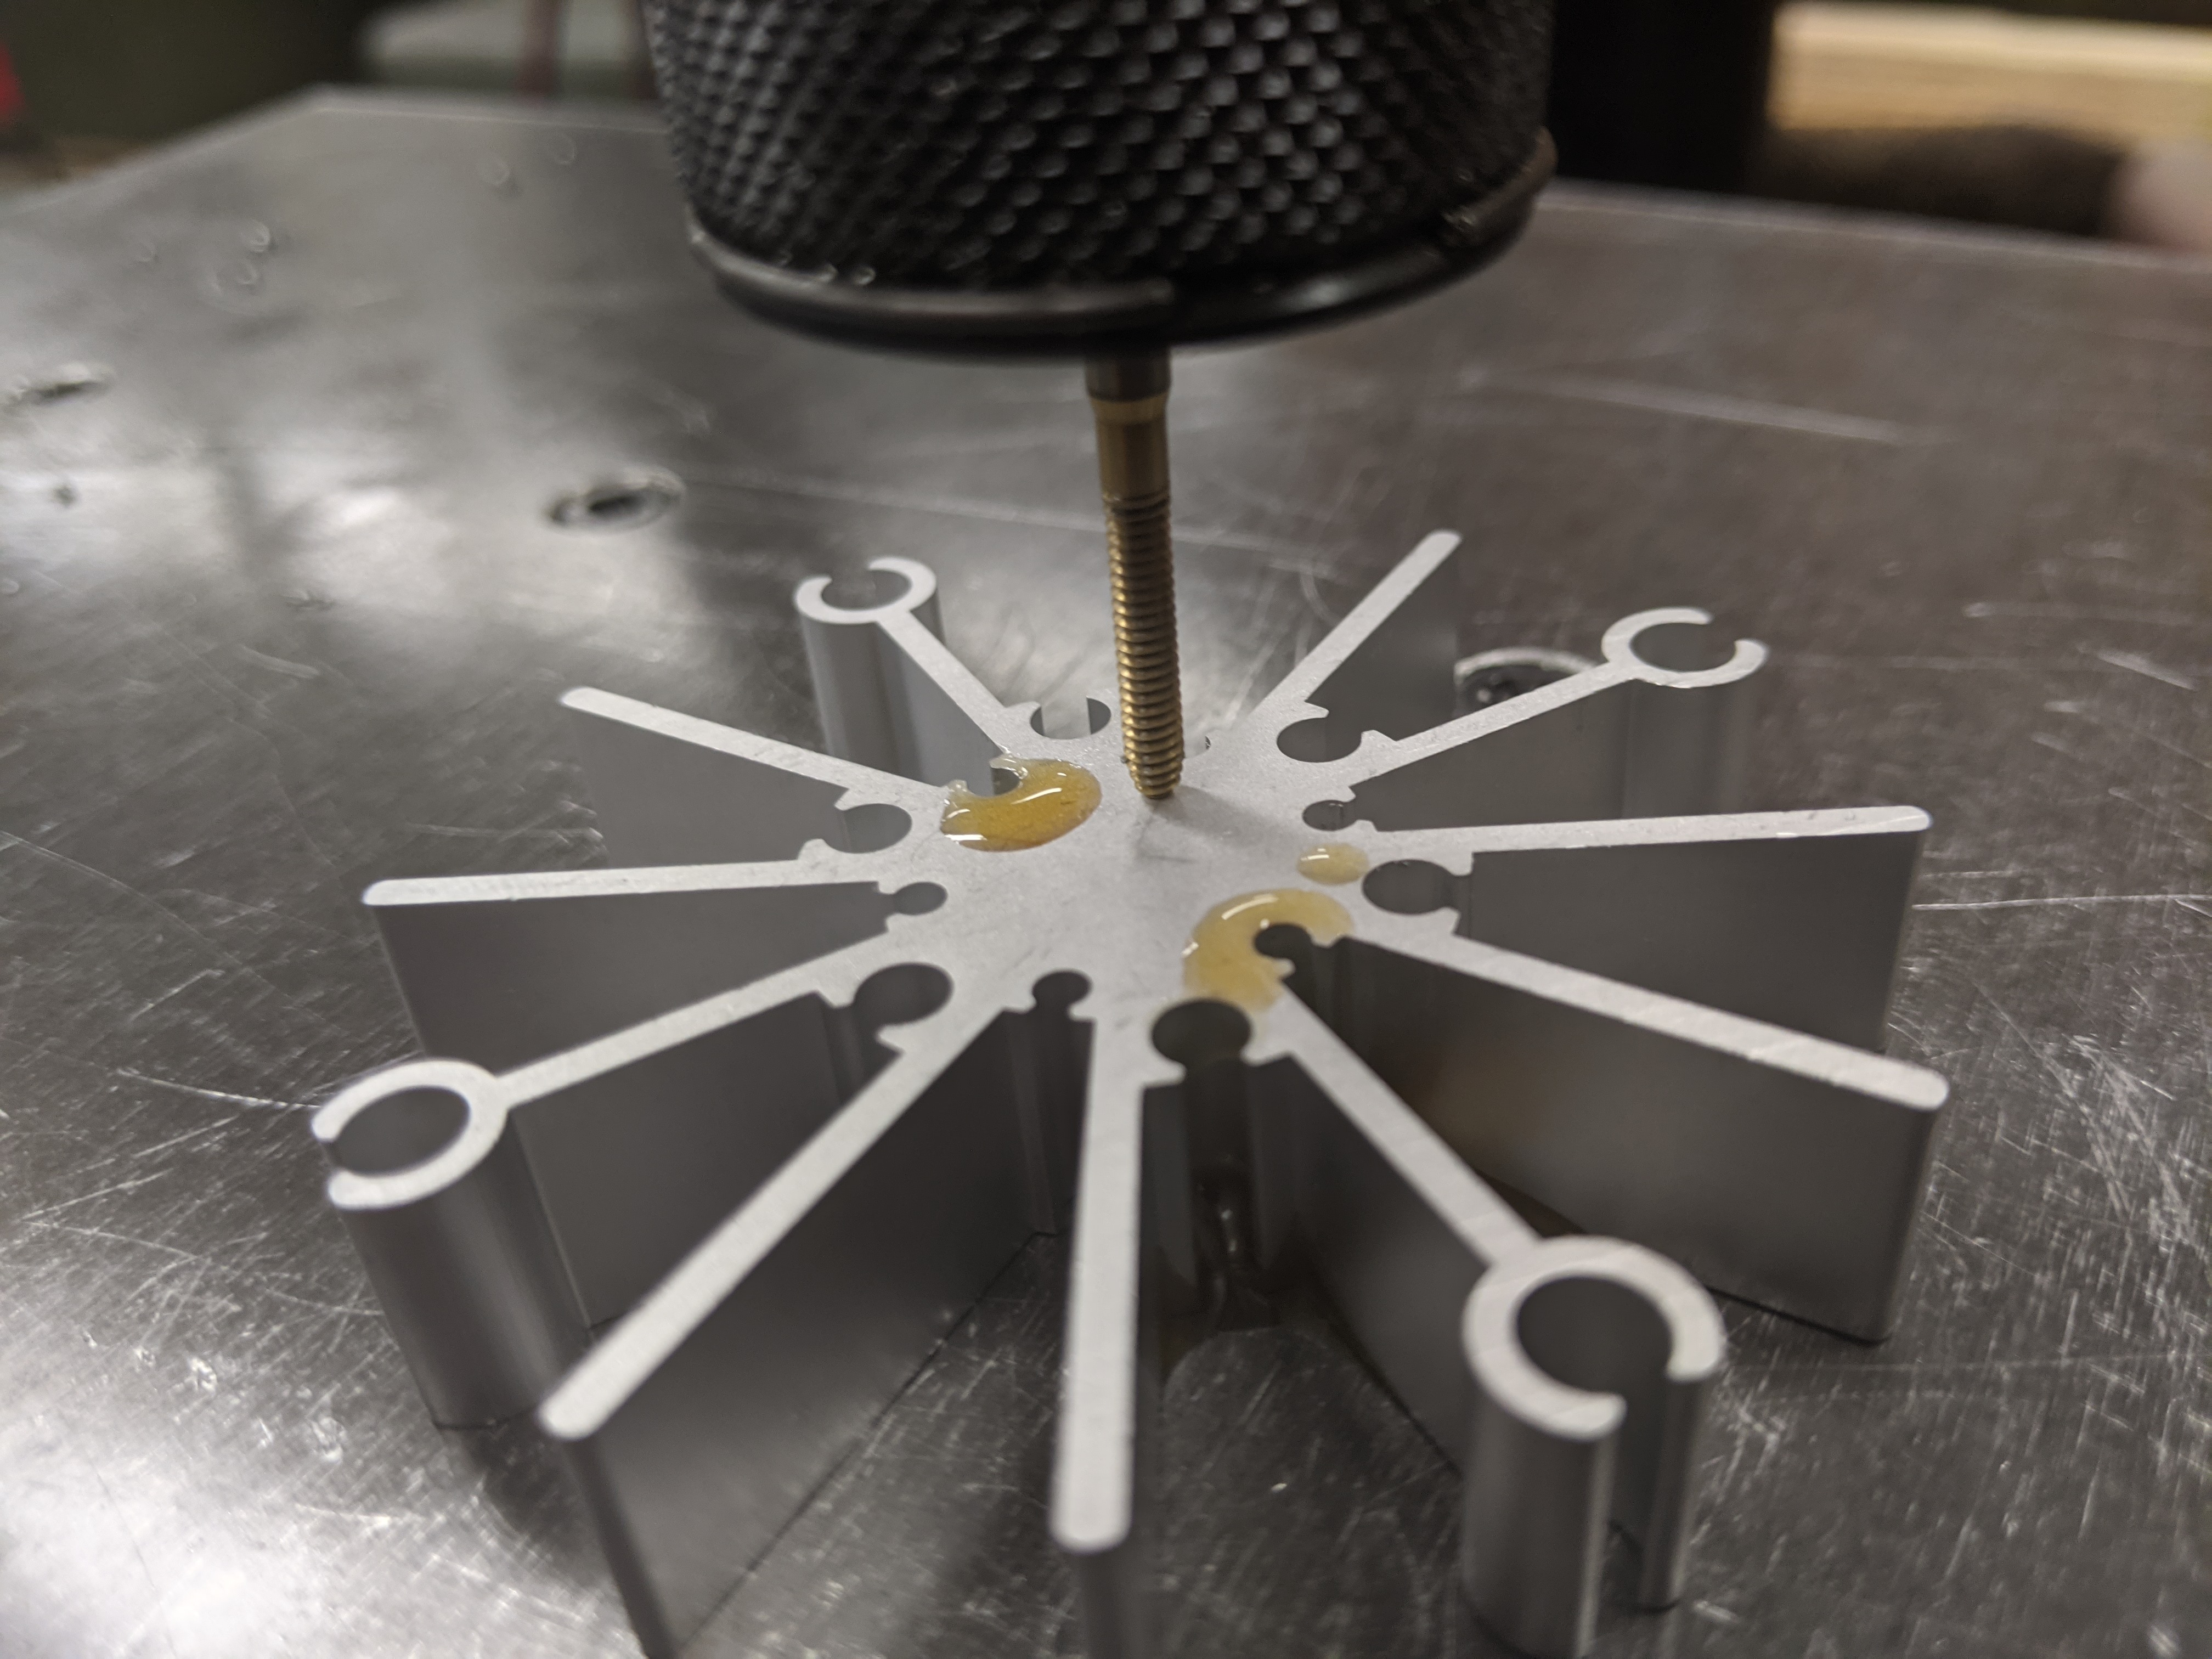
\includegraphics[width=\textwidth/2]{"./tap-heatsink.jpg"}
\end{center}

The aluminum heatsinks arrive preformed but without any tapping.
Tap the heatsink for imperial 4-40 machine screws.
We used thread-forming tap: OSG 1400105300 with a pneumatic ``air-tapper'' (pictured above), but you may do this by hand if you wish.
You will need to tap just two of the innermost holes.

\begin{center}
  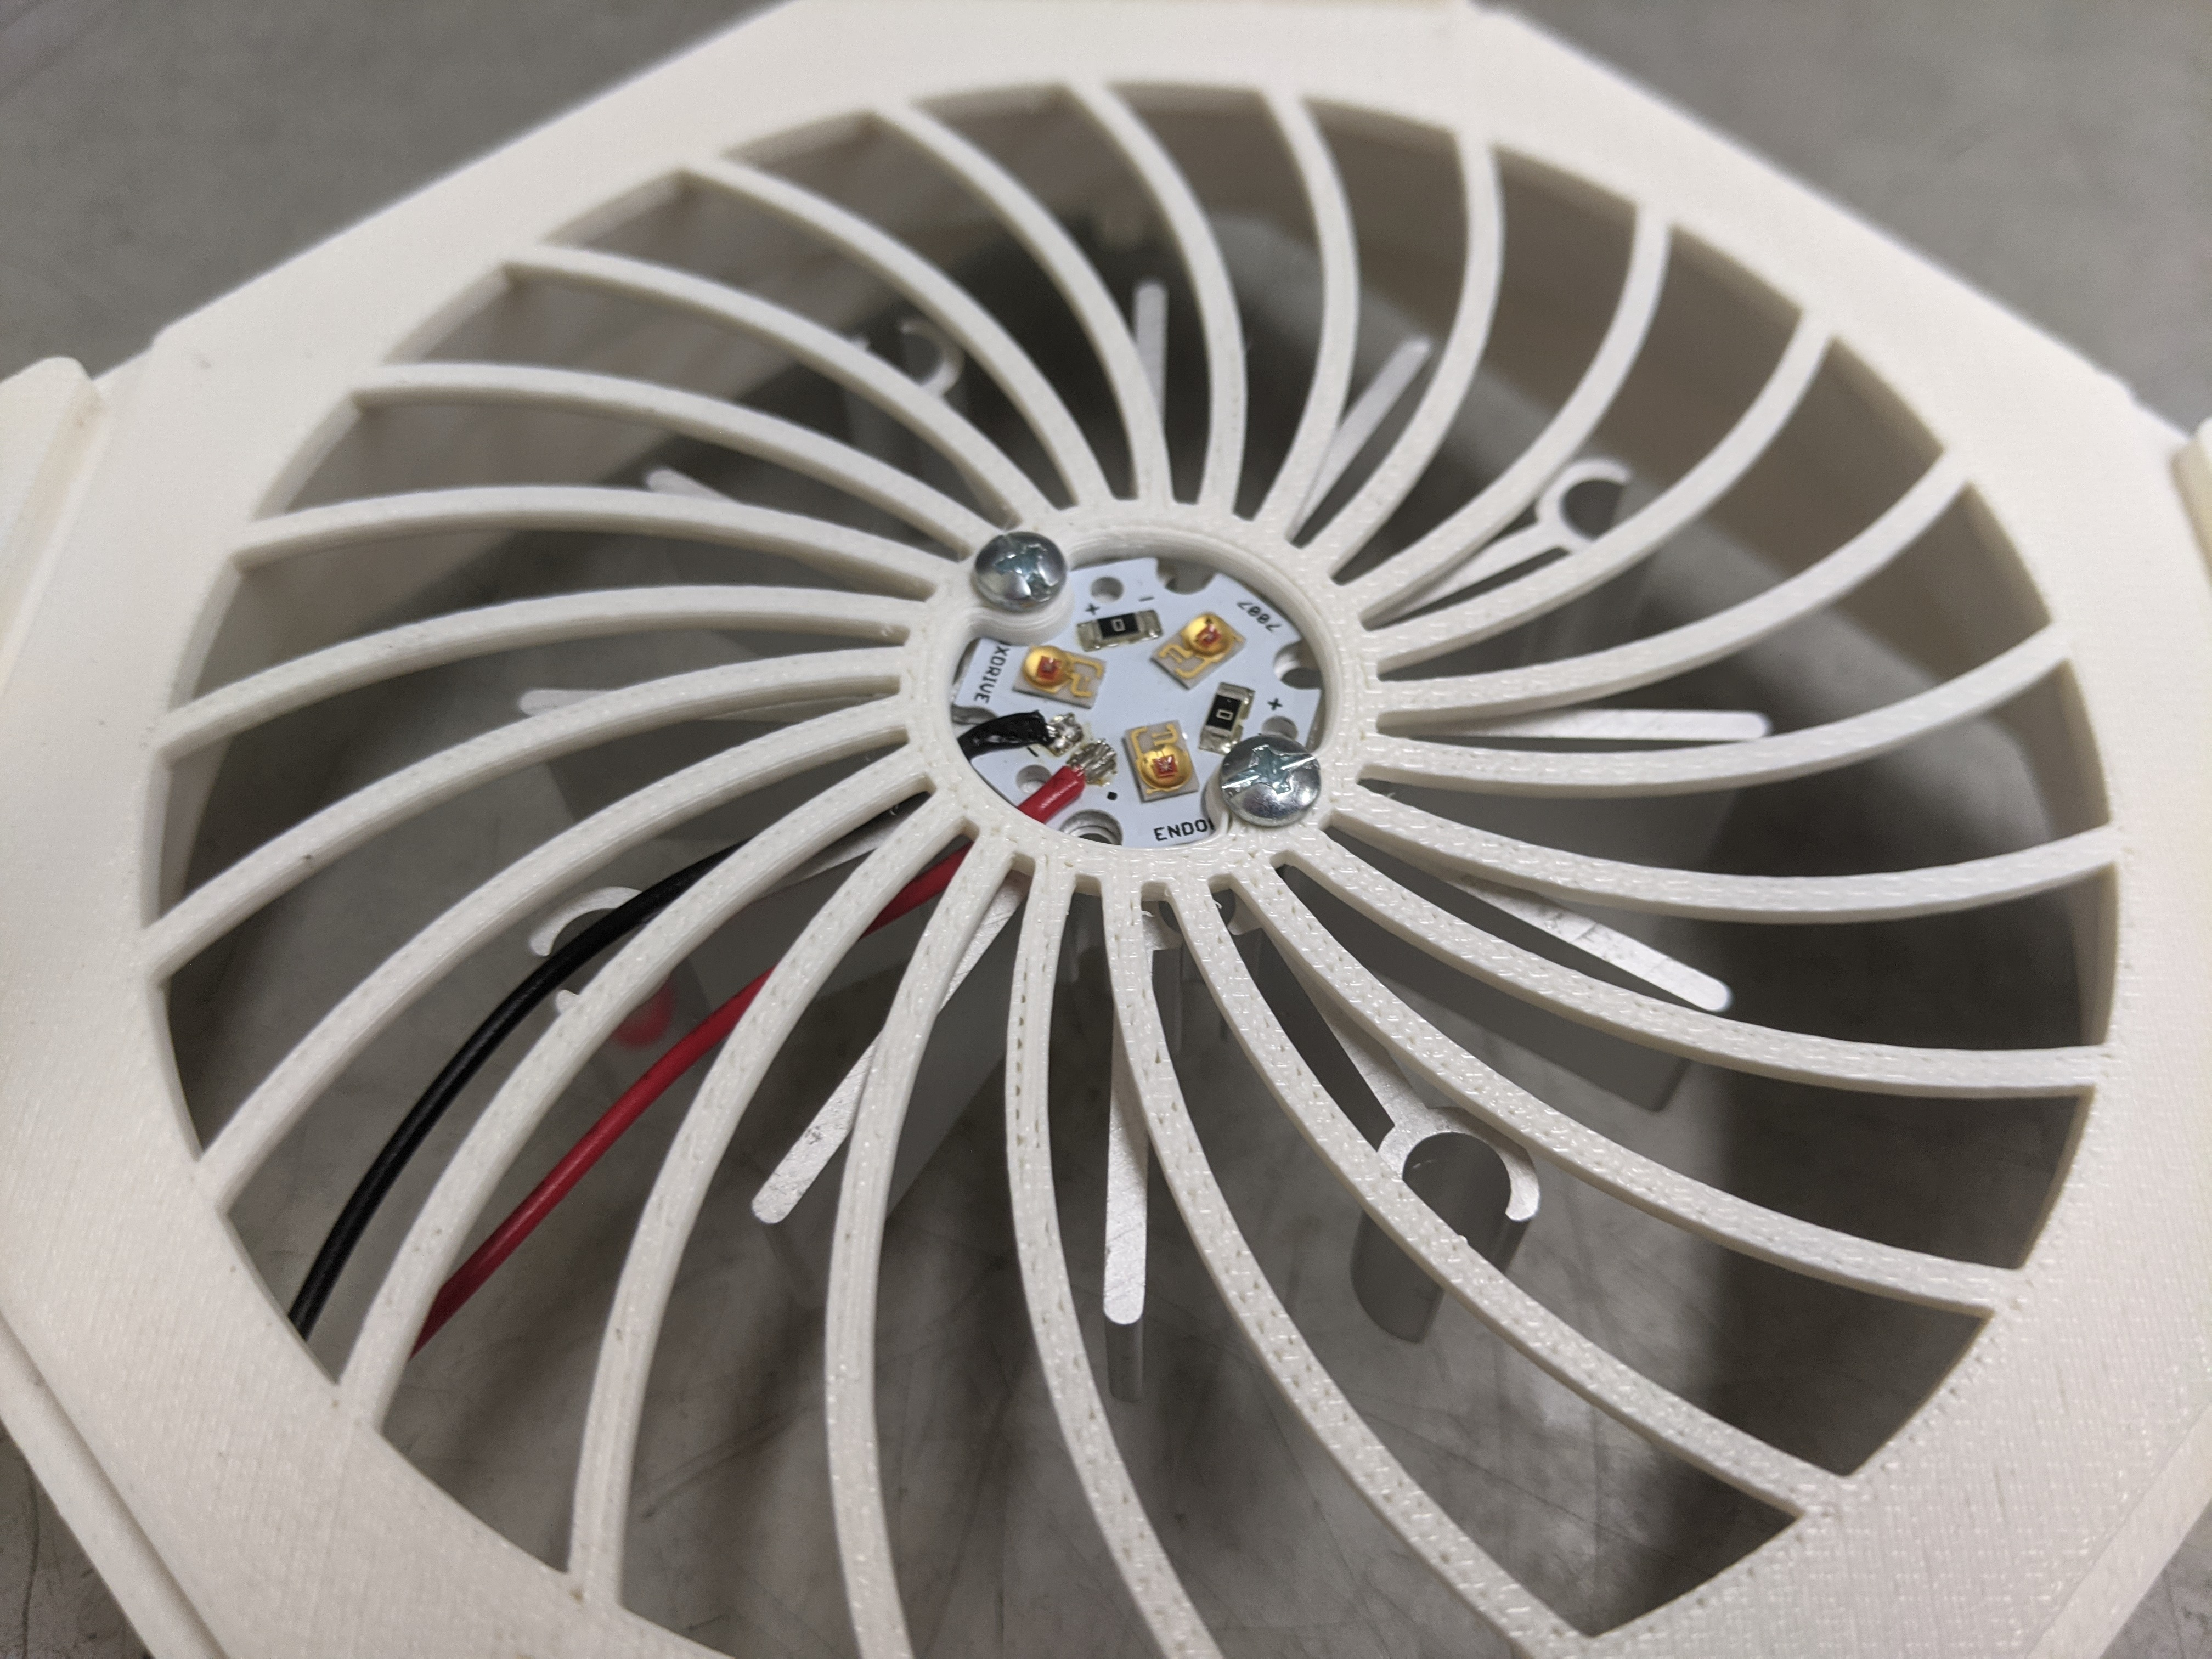
\includegraphics[width=\textwidth/2]{"./led-and-heatsink.jpg"}
\end{center}

Install the LED star and heatsink with wires facing towards printed hole.
Use 1/4'' screws.

\begin{center}
  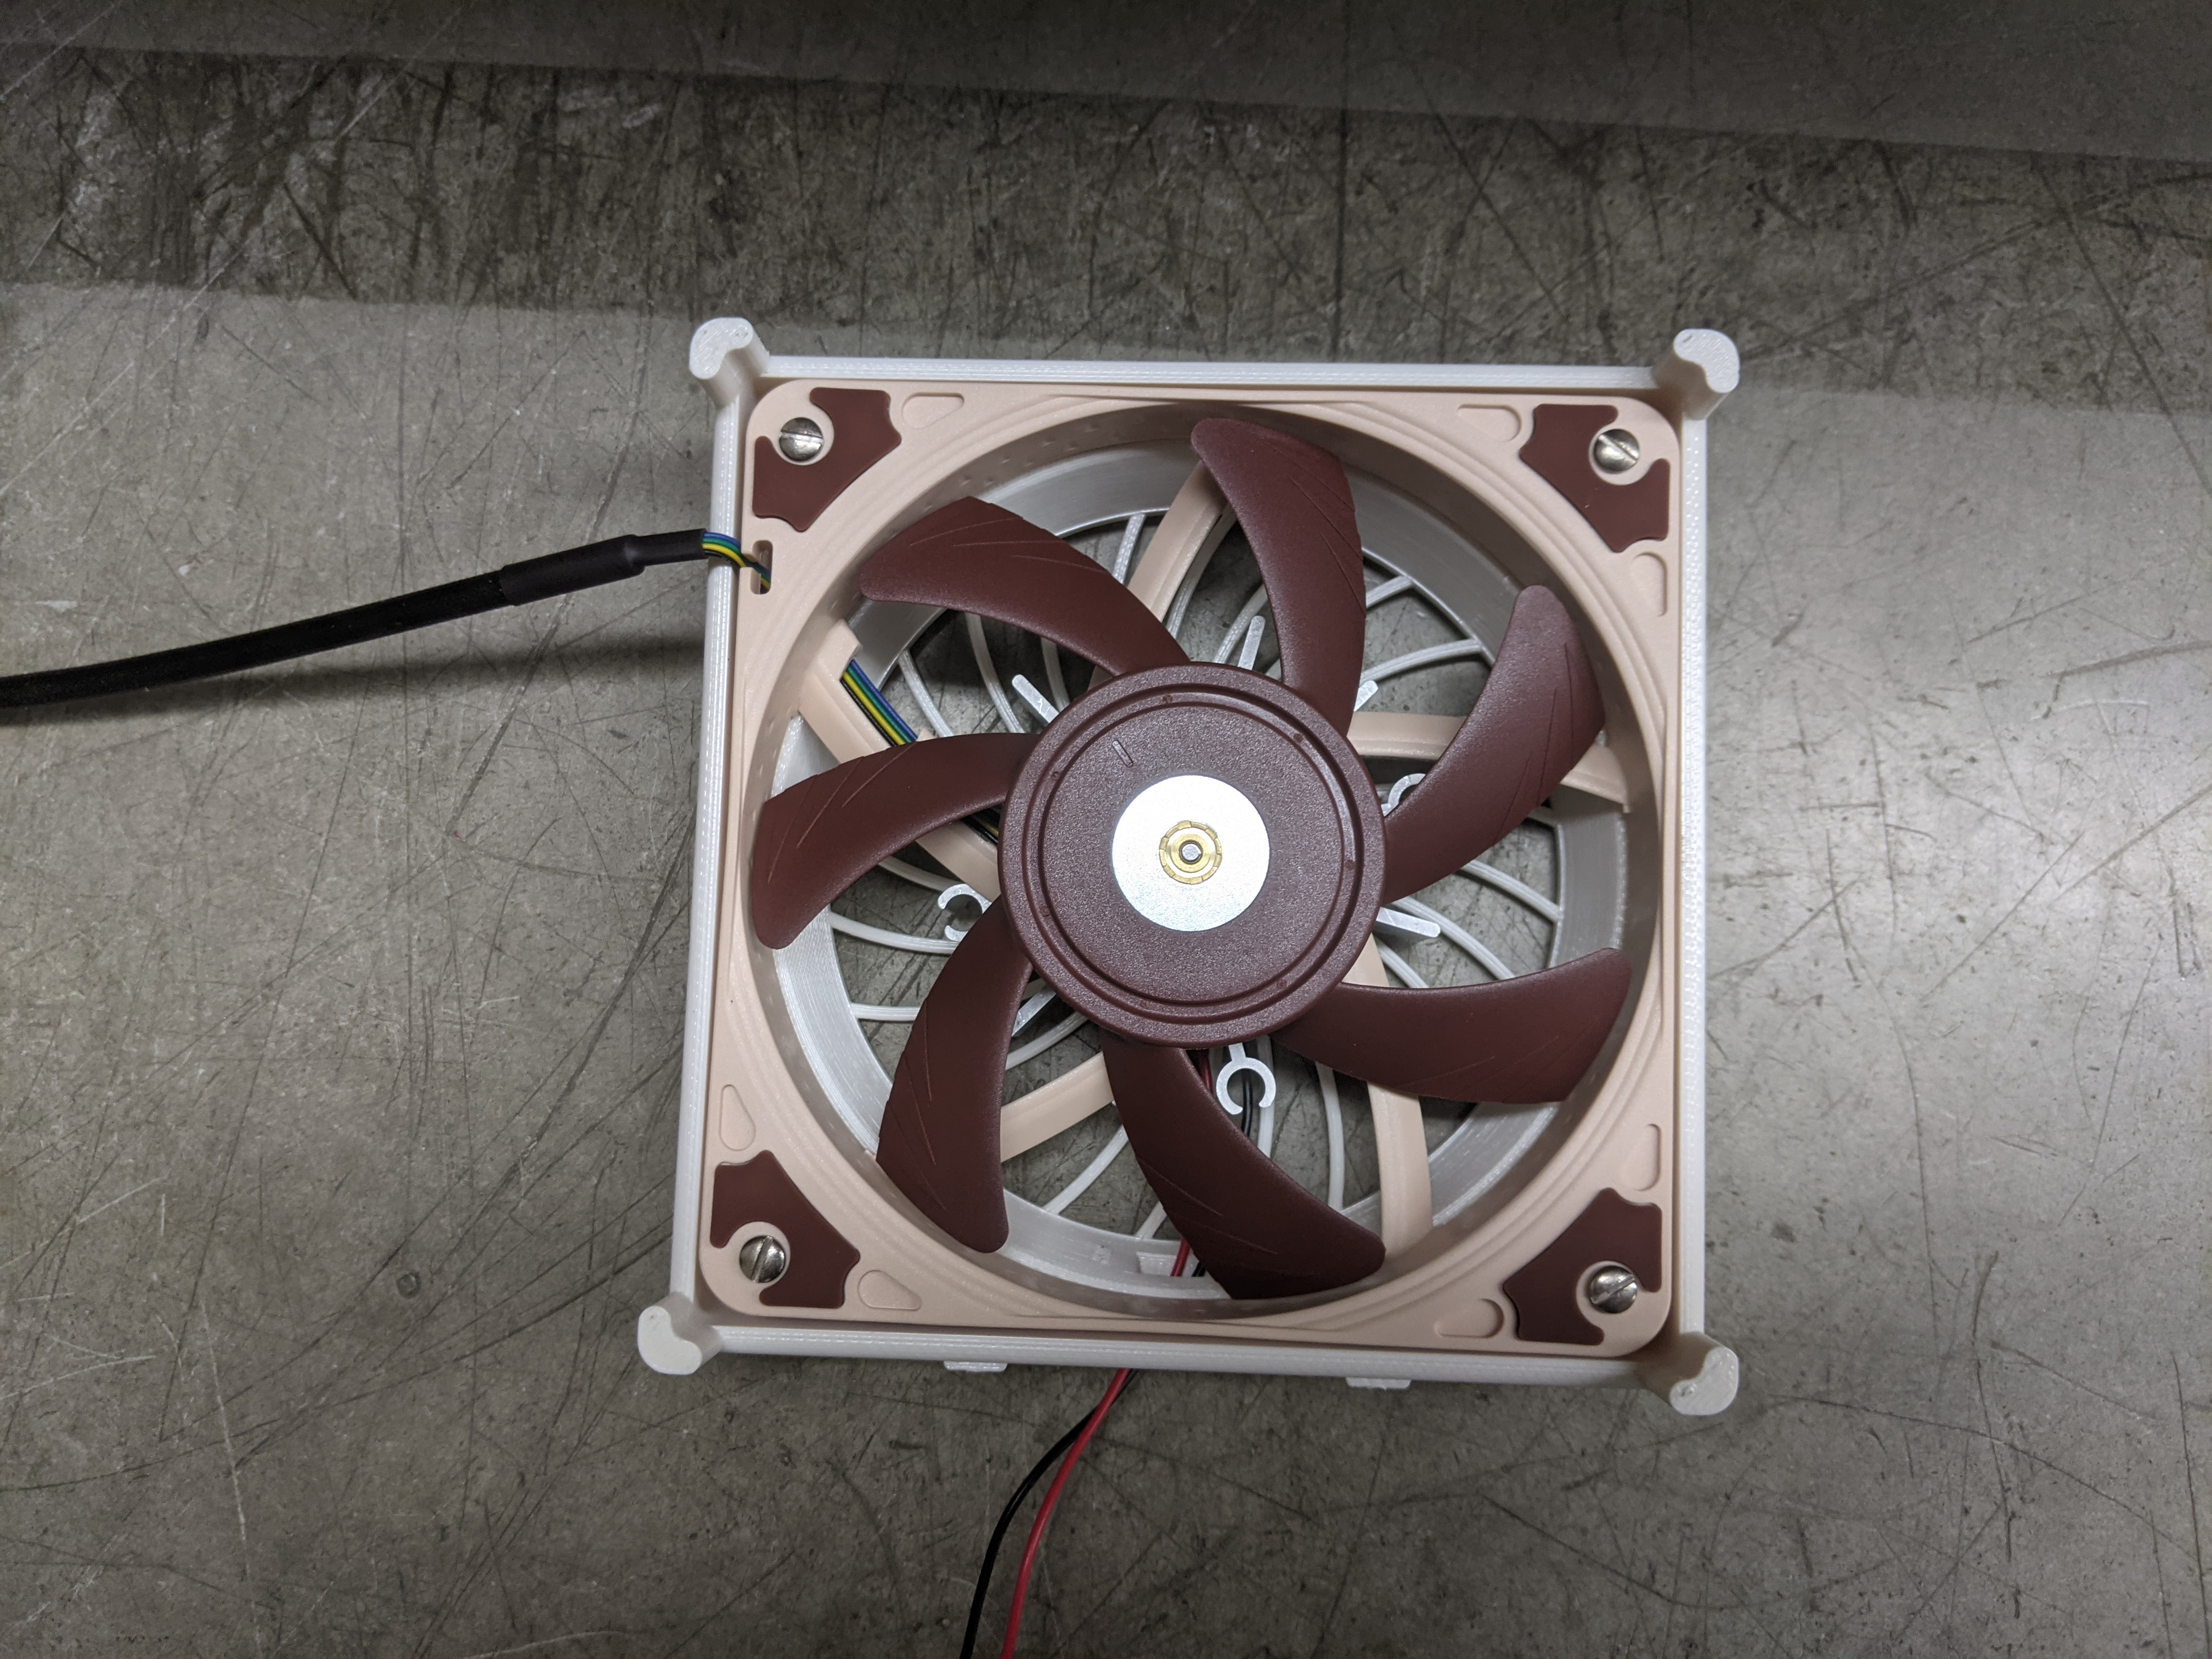
\includegraphics[width=\textwidth/2]{"./mounted-fan.jpg"}
\end{center}

Install the fan.
Pay special attention to the orientation of the fan, including the location of the cord.
Use 3/4'' screws here.

\begin{center}
  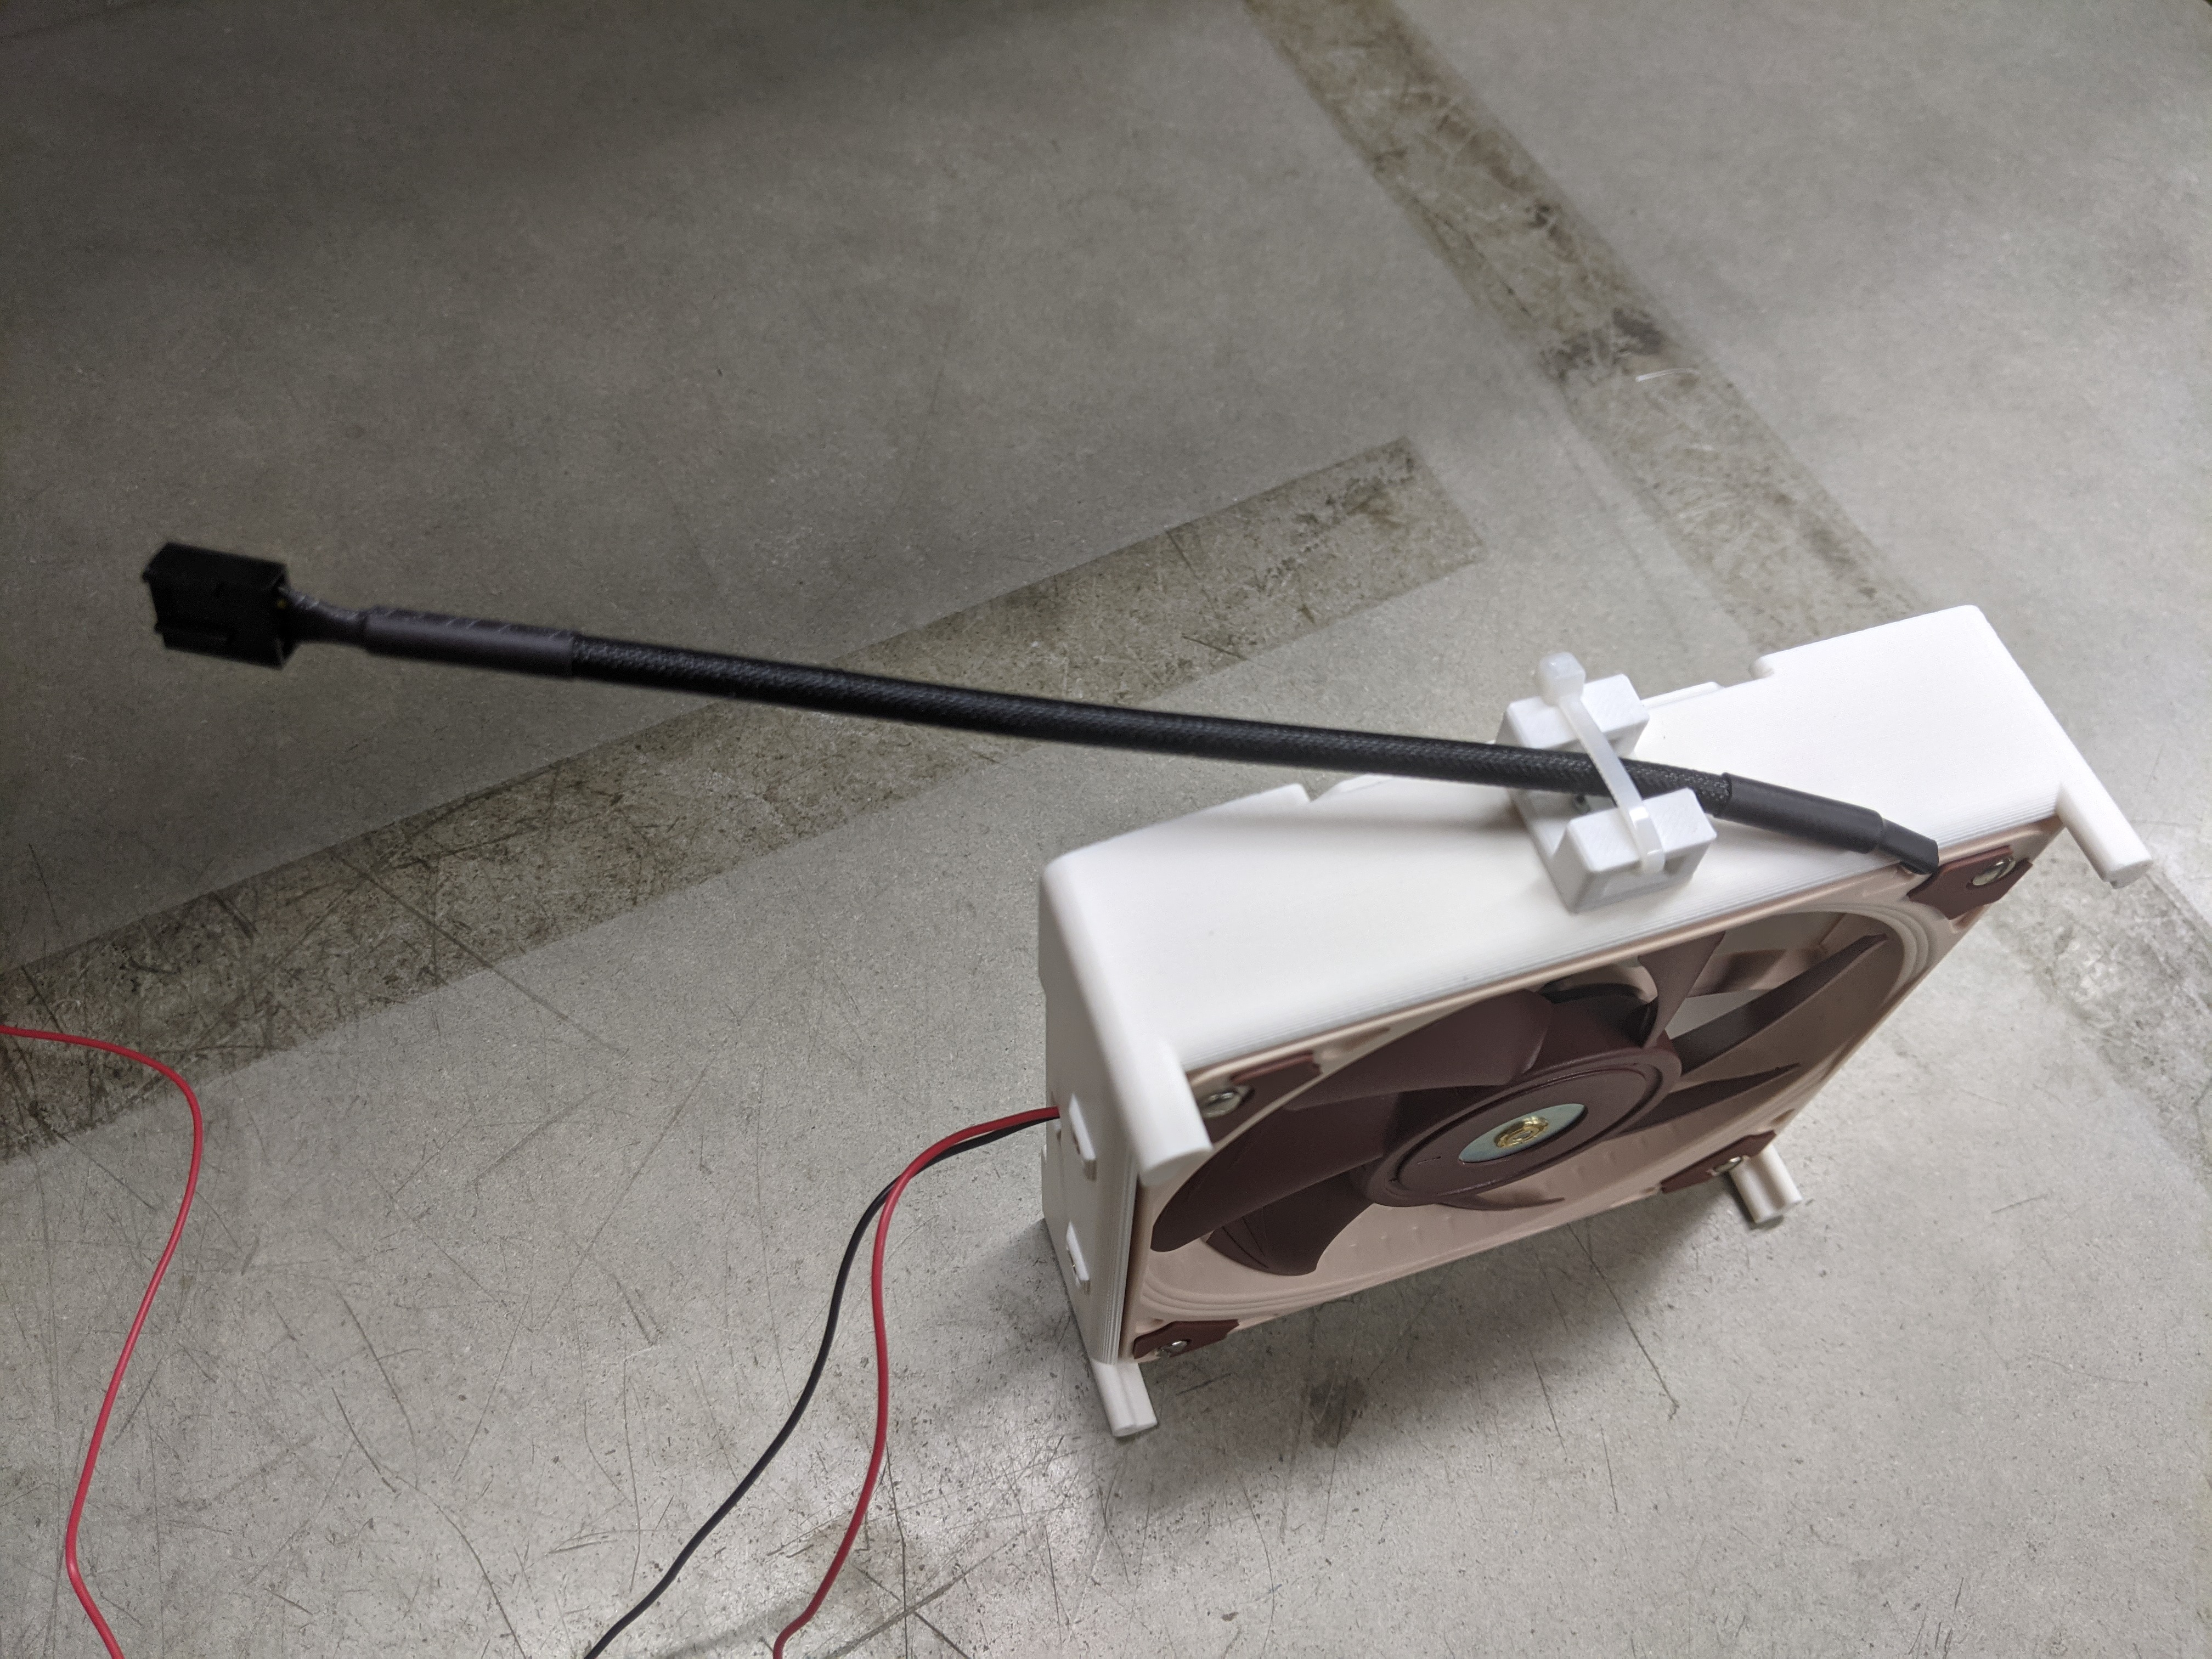
\includegraphics[width=\textwidth/2]{"./cable-tie.jpg"}
\end{center}

Install the cable anchor using a 1/4'' screw.
Use a zip tie to capture the fan cord, as shown above.

\clearpage

\begin{center}
  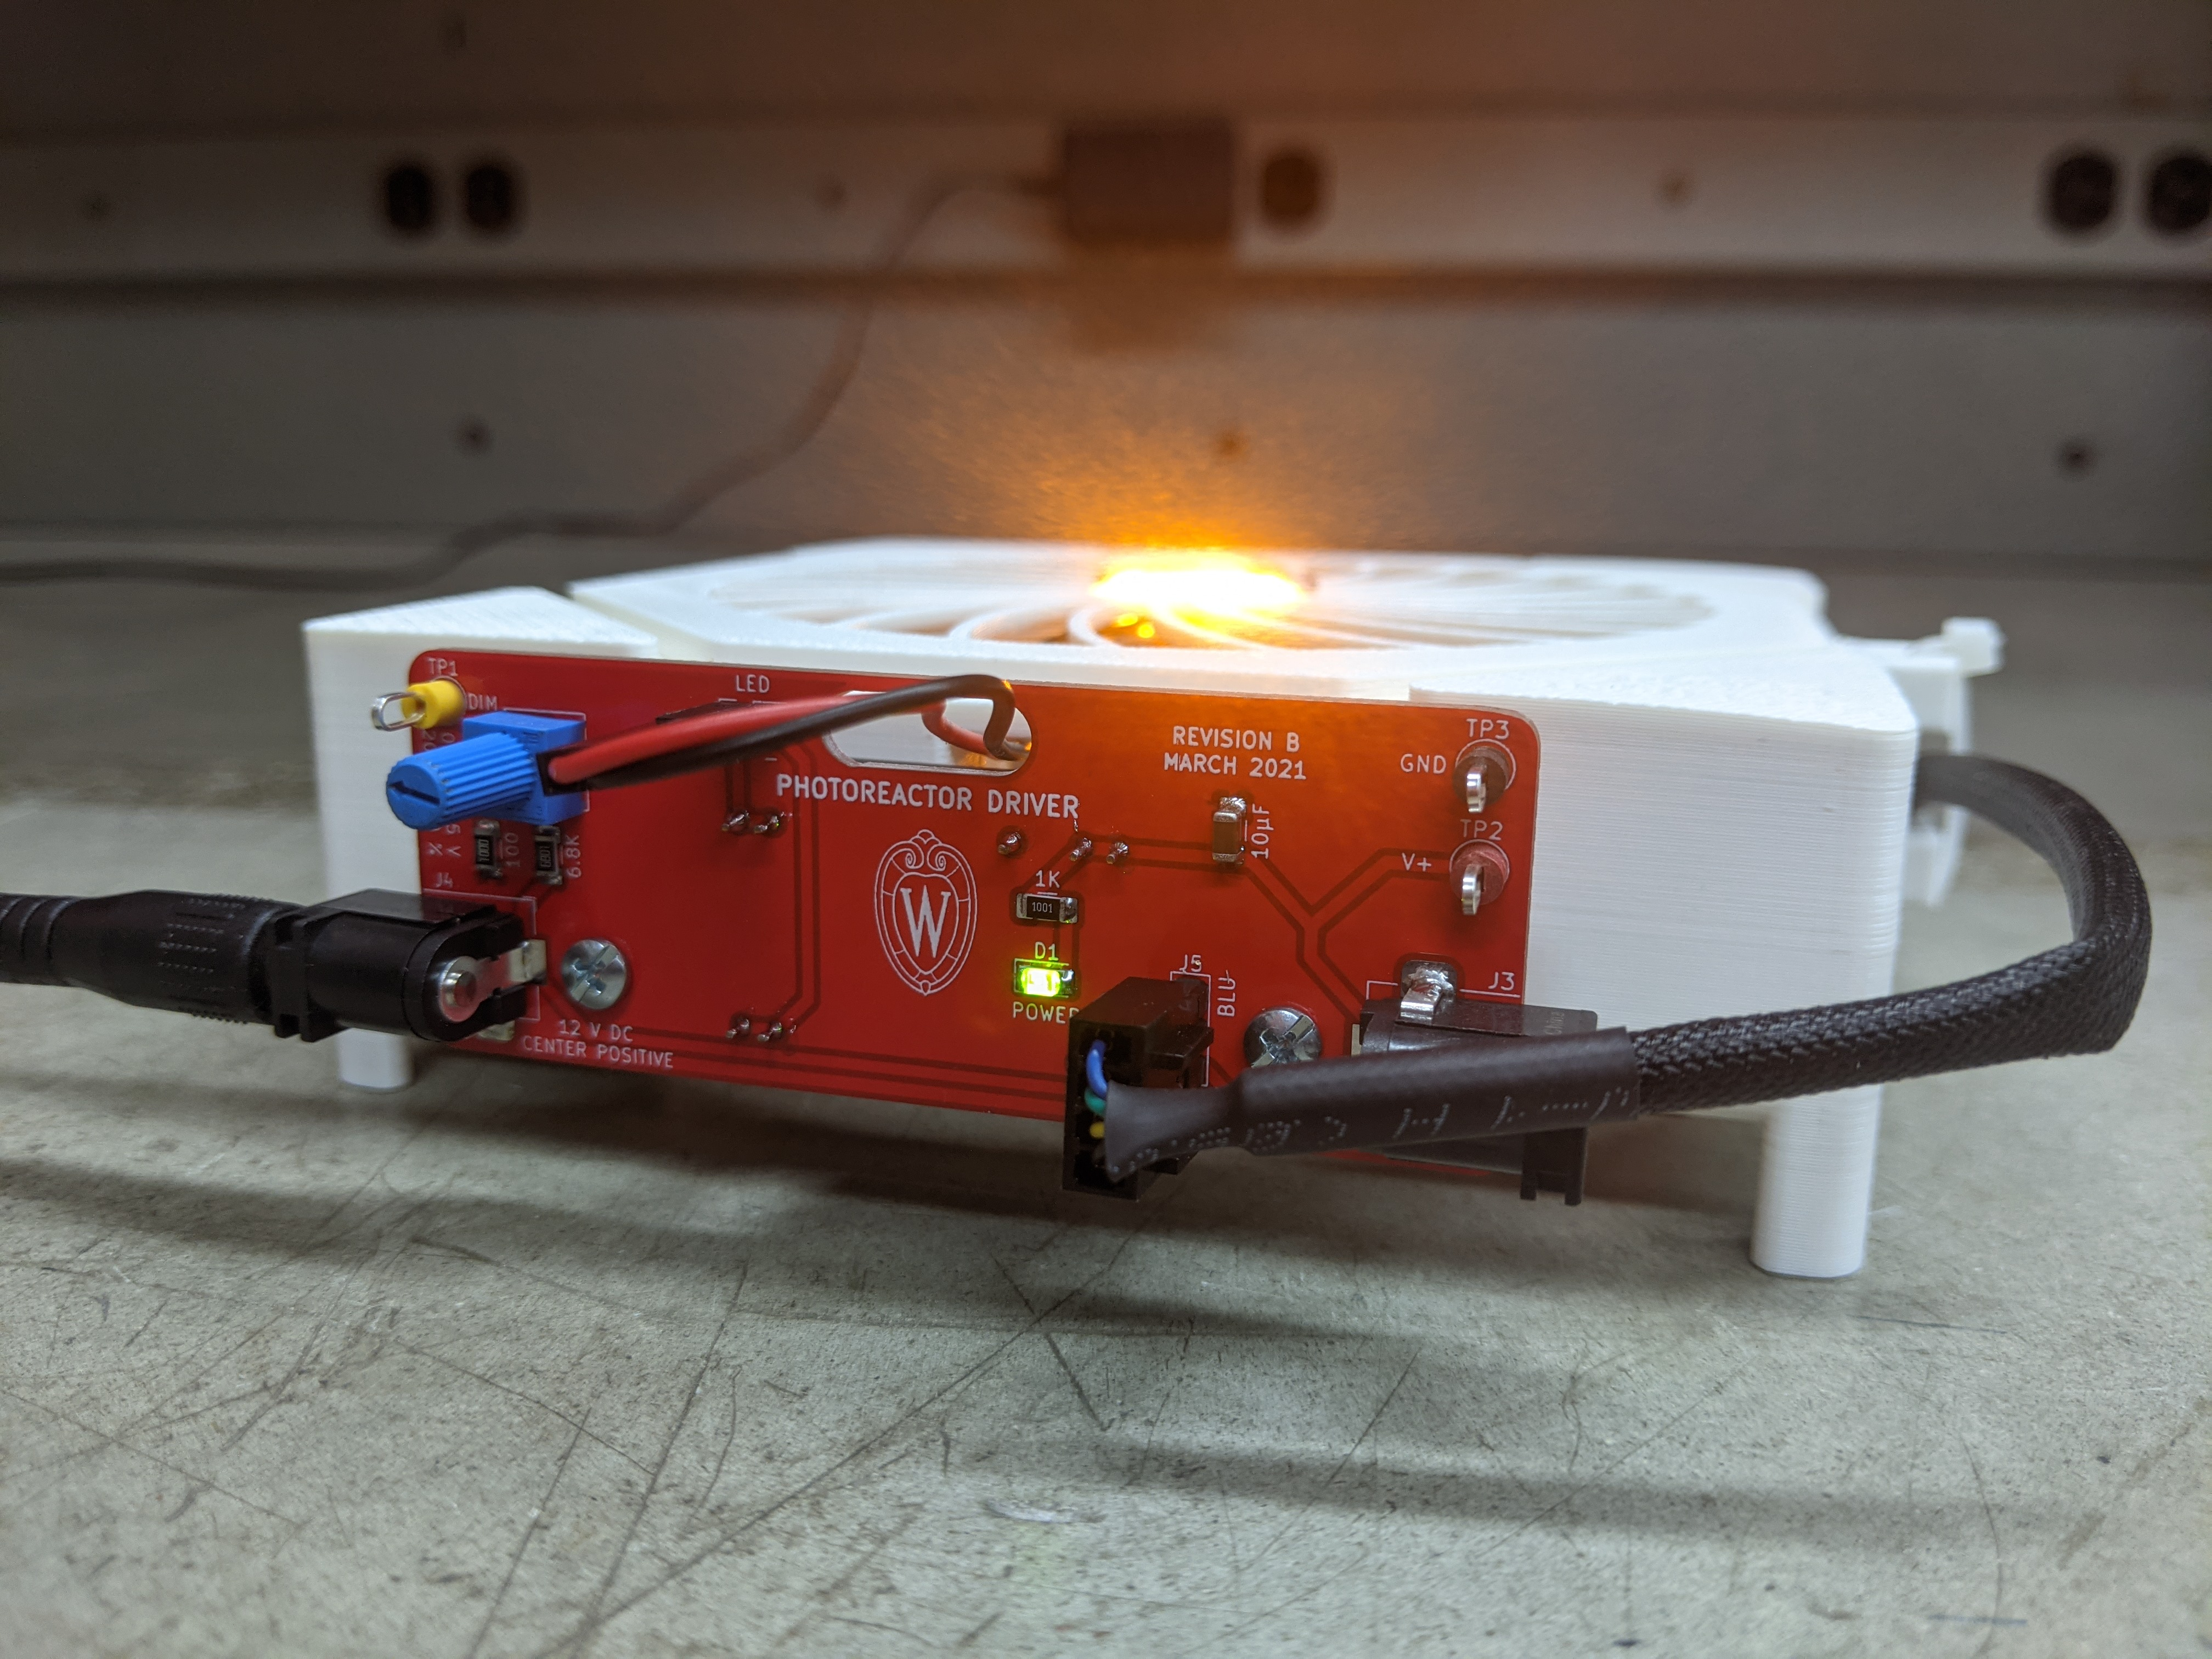
\includegraphics[width=\textwidth/2]{"./driver-on-base.jpg"}
\end{center}

Install the driver board using the threaded standoffs.
Plug the LED and fan into the board.
Pay special attention to the orientation of the fan connector.
You should now be ready to test your base---remember to use proper eye protection!

\clearpage
\subsection{Top} \label{SEC:top}

\begin{center}
  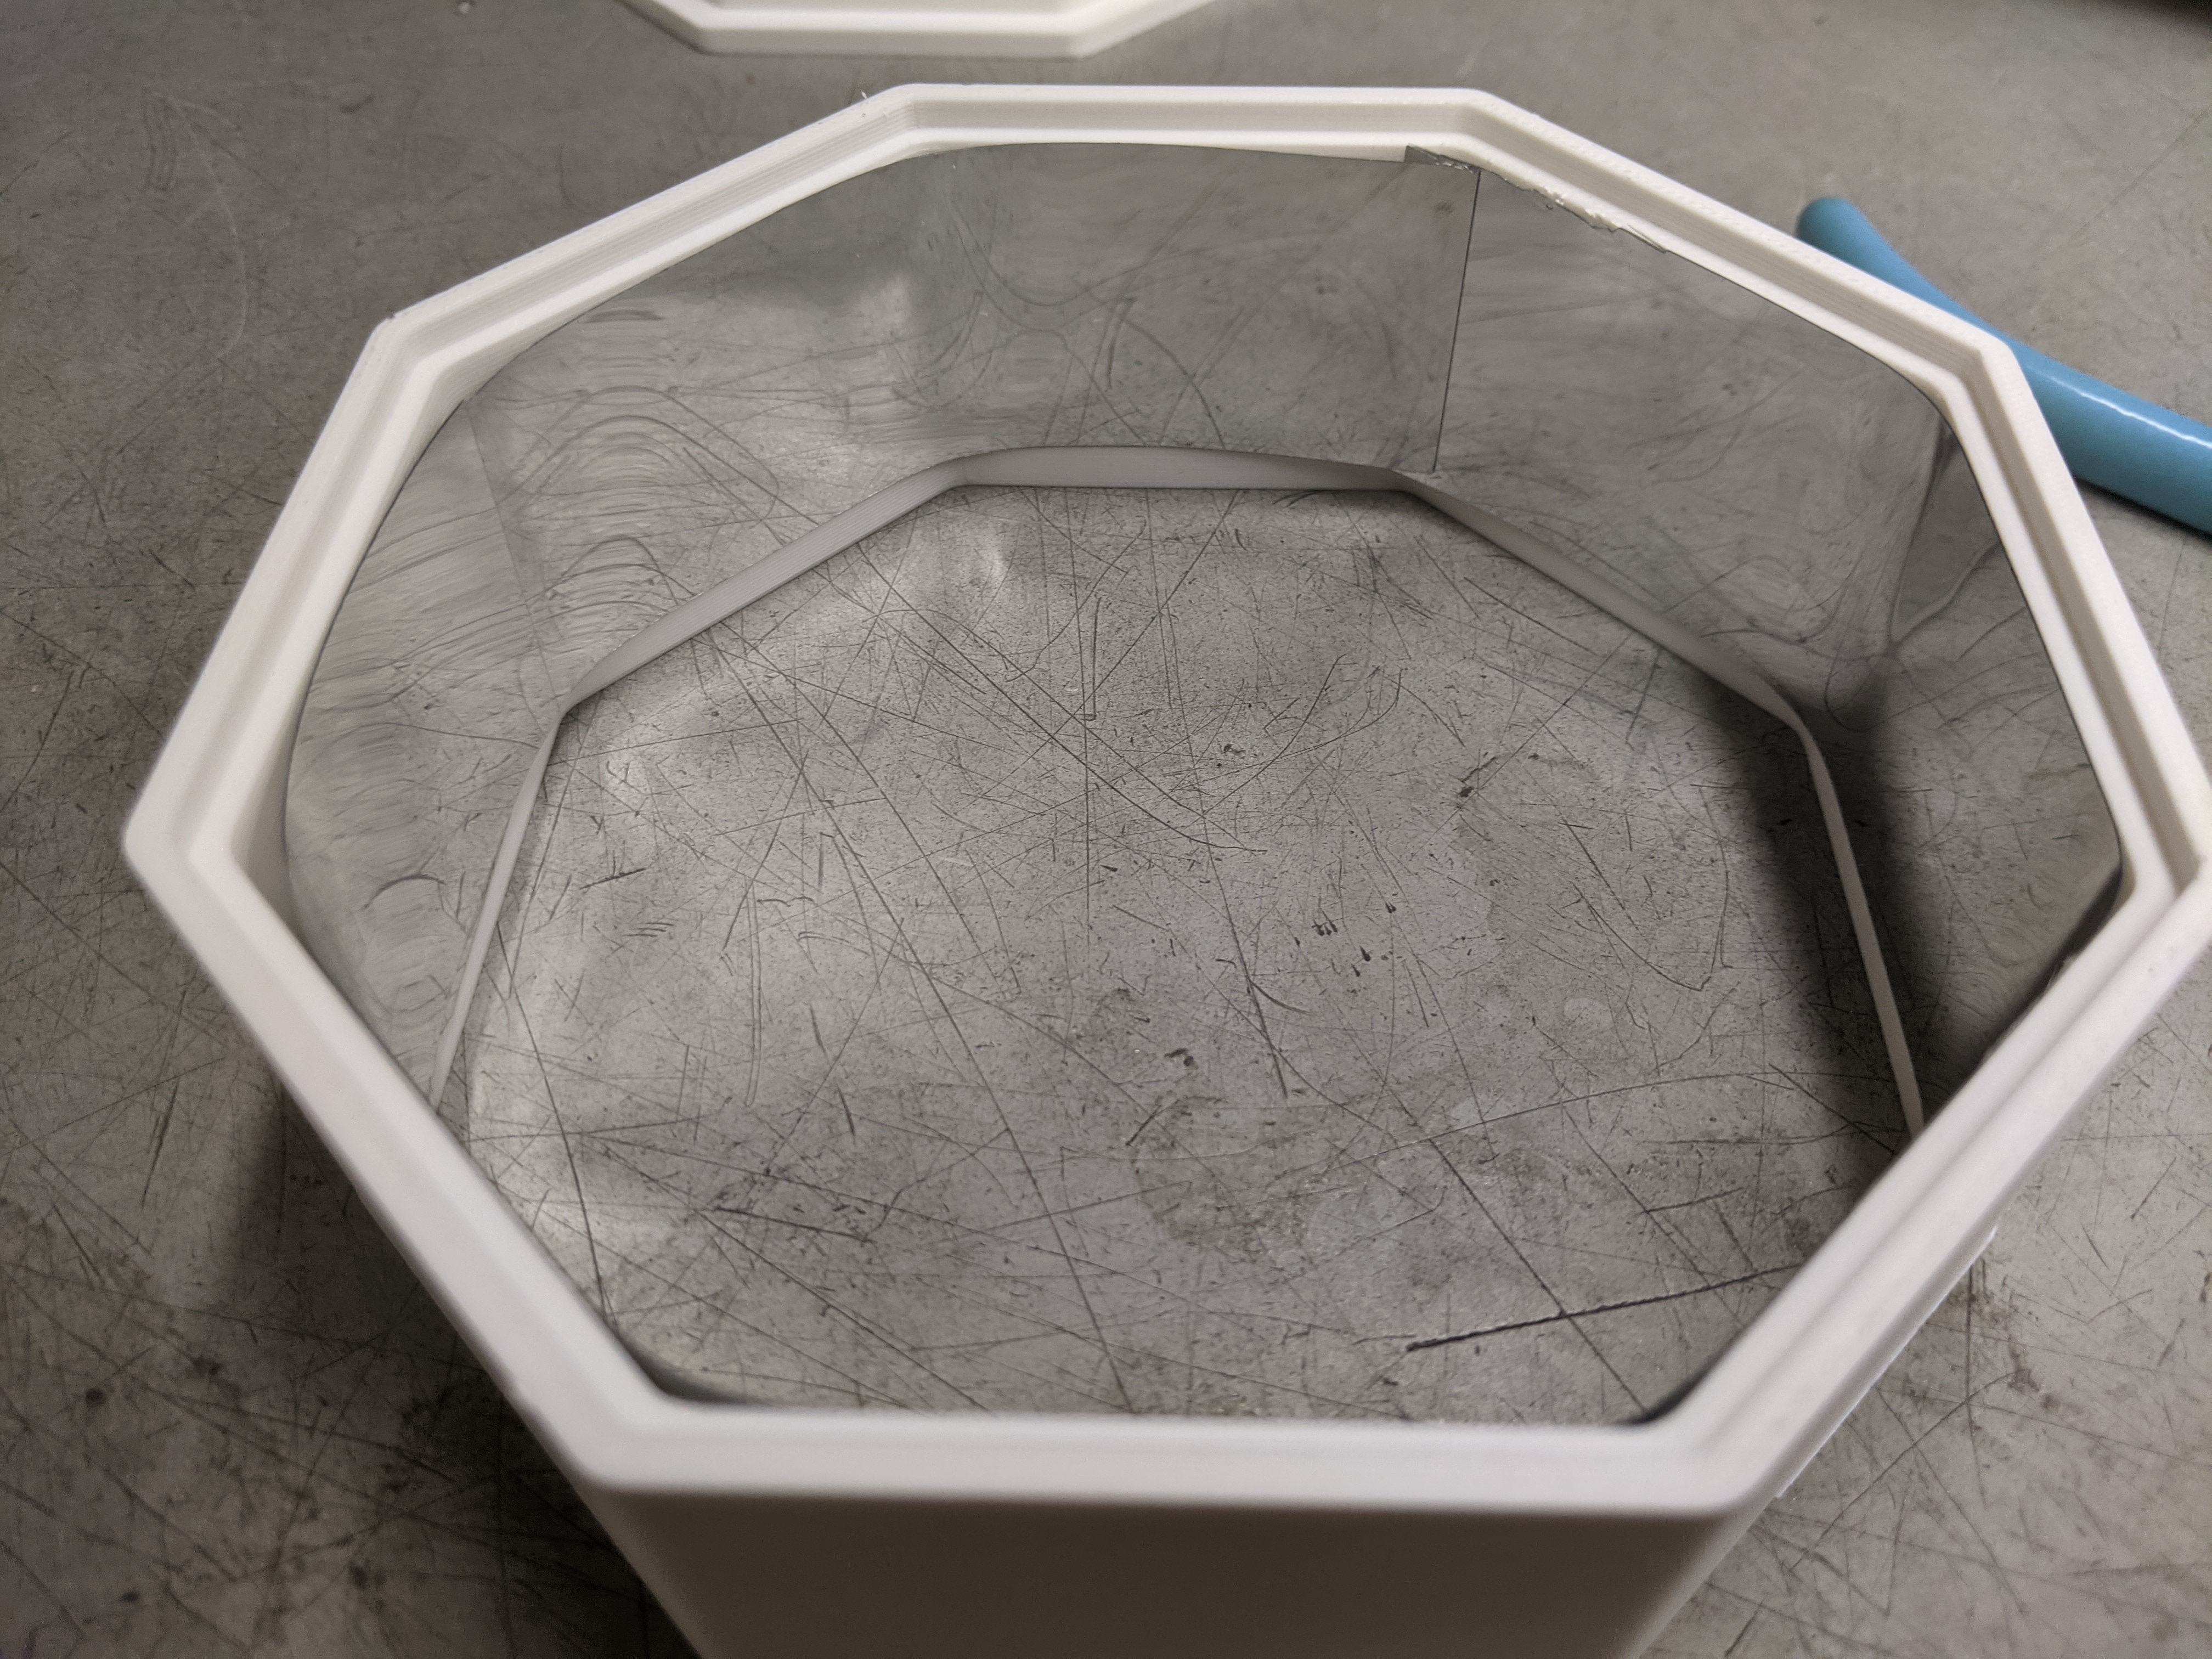
\includegraphics[width=\textwidth/2]{"./reflector.jpg"}
\end{center}

Simply cut the reflective material to line the chamber.
It's good to leave overlap around the interior, as shown.
Remove the backing and stick the material to the chamber walls.

\end{document}
